\documentclass[
    table,
    12pt,
    oneside,
    a4paper,
    italian
]{book}

\PassOptionsToPackage{dvipsnames}{xcolor} % colori PDF/A

\usepackage{colorprofiles}
% PDF/A
% validate in https://www.pdf-online.com/osa/validate.aspx
\usepackage[a-1a,mathxmp]{pdfx}[2018/12/22]
\usepackage[T1]{fontenc}
\usepackage[utf8]{inputenc}
\usepackage[italian]{babel}
\usepackage{bookmark}
\usepackage{caption}
\usepackage{comment}
\usepackage{chngpage, calc} % centra il frontespizio
\usepackage{emptypage} % pagine vuote senza testatina e piede di pagina
\usepackage{epigraph} % per epigrafi
\usepackage{indentfirst} % rientra il primo paragrafo di ogni sezione
\usepackage{graphicx} % immagini
\usepackage[pdfa]{hyperref} % collegamenti ipertestuali
\usepackage{mparhack,relsize}  % finezze tipografiche
\usepackage{nameref} % visualizza nome dei riferimenti
\usepackage[font=small]{quoting} % citazioni
\usepackage{subfig} % sottofigure, sottotabelle
\usepackage[italian]{varioref} % riferimenti completi della pagina
\usepackage{longtable} % tabelle su più pagine
\usepackage[toc, acronym, automake]{glossaries}
\usepackage[backend=biber, style=verbose-ibid, hyperref, backref]{biblatex}
\usepackage{lmodern}
\usepackage[top=2.75cm, bottom=2.75cm, right=3cm, left=3cm]{geometry} % 1in+17pt+0.6cm
%\usepackage[top=2.75cm, bottom=2.75cm, right=3cm, left=3.75cm]{geometry} % 1in+17pt+0.6cm
\usepackage{fancyhdr}
\usepackage{lipsum}
\usepackage{setspace}
\usepackage{titlesec}
\usepackage{minted} % https://it.overleaf.com/learn/latex/Code_Highlighting_with_minted
\usepackage{xcolor}
\usepackage{csquotes} % gestisce automaticamente i caratteri (")
\usepackage{etoolbox}
\usepackage{dirtree}
% Load variables
\newcommand{\myUni}{Università degli Studi di Padova}
\newcommand{\myDepartment}{Dipartimento di Matematica ``Tullio Levi-Civita''}
\newcommand{\myFaculty}{Corso di Laurea in Informatica}
\newcommand{\myTitle}{Lorem ipsum dolor sit amet, consectetur adipisci elit.}
\newcommand{\myDegree}{Tesi di Laurea Triennale}
\newcommand{\profTitle}{Prof.}
\newcommand{\myProf}{Cognome Nome}
\newcommand{\graduateTitle}{Laureando}
\newcommand{\myName}{Bobirica Andrei Cristian}
\newcommand{\myStudentID}{1224449}
\newcommand{\myAA}{2023-2024}
\newcommand{\myLocation}{Padova}
\newcommand{\myTime}{Luglio 2024}
% Glossary
\newacronym{ddc}{DDC}{Data Driven Cooking}
\newglossaryentry{ddcg}{
    name={DDC},
    text={Data Driven Cooking},
    sort=ddc,
    description={Una piattaforma di cucina intelligente che utilizza i dati per ottimizzare e migliorare i processi di cottura. DDC fornisce funzionalità avanzate per i proprietari di forni, consentendo loro di monitorare e controllare i dispositivi in modo efficiente}
}

\newacronym{rtk}{RTK}{Redux Toolkit}
\newglossaryentry{rtkg}{
    name={RTK},
    text={Redux Toolkit},
    sort=rtk,
    description={Un toolkit per Redux che semplifica la scrittura della logica Redux e automatizza configurazioni complesse. RTK è stato utilizzato per gestire lo stato globale dell'applicazione in modo efficiente e strutturato}
}

\newacronym{cicd}{CI/CD}{continuous integration and continuous delivery}
\newglossaryentry{cicdg}{
    name={CI/CD},
    text={CI/CD},
    sort=cicd,
    description={Integrazione continua e consegna continua. L'integrazione continua (CI) è una pratica di sviluppo software in cui i membri del team integrano il loro lavoro frequentemente, con verifiche automatizzate per rilevare errori rapidamente. La consegna continua (CD) estende la CI, automatizzando ulteriormente il processo di rilascio per consentire la distribuzione di software in produzione in modo rapido e affidabile.}
}


\newglossaryentry{ddcserviceg}{
    name={DDC Service},
    sort=ddcservice,
    description={Un'applicazione destinata al personale tecnico e di manutenzione dei forni, offrendo strumenti avanzati per la gestione e il supporto dei dispositivi. DDC Service facilita la risoluzione dei problemi e l'ottimizzazione delle operazioni di servizio}
}

\newglossaryentry{servicedoveng}{
    name={Serviced Oven},
    sort=servicedoven,
    description={Nel contesto della applicazione DDC Service per Serviced Oven si intente un prodotto, in particolare un forno. Questo forno è un prodotto a cui un addetto Service presta servizzi di assistenza e riparazione. Un Utente Autenticato della app DDC Service ha tra i sui Serviced Ovens i prodotti a cui presta assistenza e servizi di Service. Un Serviced Oven è un prodotto fisico realmente esistente edentificato da un seriale.}
}

\newglossaryentry{productcodeg}{
    name={Product Code},
    sort=productcode,
    description={Un identificativo univoco assegnato a ogni prodotto per la tracciabilità e la gestione. Utilizzato nelle applicazioni per monitorare e gestire specifici modelli di forni}
}

\newglossaryentry{firmwareg}{
    name={Firmware},
    sort=firmware,
    description={Il software integrato nei dispositivi hardware, come i forni, che gestisce le loro operazioni fondamentali. Gli aggiornamenti del firmware migliorano le prestazioni e aggiungono nuove funzionalità ai dispositivi}
}

\newglossaryentry{navbarg}{
    name={Nav Bar},
    sort=navbar,
    description={La barra di navigazione dell'applicazione che consente agli utenti di accedere rapidamente alle diverse sezioni e funzionalità}
}

\newglossaryentry{tabbarg}{
    name={Tab Bar},
    sort=tabbar,
    description={Una barra di navigazione a schede che permette agli utenti di passare facilmente tra diverse schermate o funzionalità dell'applicazione}
}

\newglossaryentry{ecng}{
    name={ECN},
    sort=ecn,
    description={Per ECN si intende un codice che identifica il versionamente di uno specifico forno, un diverso versionamento potrebbe indicare caratteristiche diverse di un medesimo prodotto}
}

\newacronym{e2e}{E2E}{End To End}
\newglossaryentry{e2eg}{
    name={E2E},
    text={End To End},
    sort=e2e,
    description={Un tipo di test che verifica il funzionamento completo di un'applicazione dal punto di vista dell'utente finale, garantendo che tutte le componenti interagiscano correttamente}
}

\newglossaryentry{designsystemg}{
    name={Design System},
    sort=designsystem,
    description={Un insieme di linee guida, componenti riutilizzabili e strumenti per creare un'interfaccia utente coerente e unificata. Il Design System garantisce uniformità visiva e comportamentale in tutte le parti dell'applicazione}
}

\newglossaryentry{frontendg}{
    name={Frontend},
    sort=frontend,
    description={La parte dell'applicazione con cui gli utenti interagiscono direttamente. Comprende l'interfaccia utente e la logica di presentazione}
}

\newglossaryentry{backendg}{
    name={Backend},
    sort=backend,
    description={La parte dell'applicazione che gestisce la logica di business, il database, e le operazioni di server. Il backend supporta il frontend fornendo dati e funzionalità}
}

\newacronym{repo}{Repo}{Repository}
\newglossaryentry{repog}{
    name={Repo},
    text={Repository},
    sort=repo,
    description={Un archivio centralizzato dove il codice sorgente e altri file di un progetto vengono memorizzati e gestiti, spesso utilizzato con sistemi di controllo versione come Git}
}

\newacronym{rma}{RMA}{Return Merchandise Authorization}
\newglossaryentry{rmag}{
    name={RMA},
    text={Return Merchandise Authorization},
    sort=rma,
    description={Un processo che consente ai clienti di restituire prodotti difettosi o non conformi per la riparazione, la sostituzione o il rimborso}
}

\newacronym{devops}{DevOps}{Development and Operations}
\newglossaryentry{devopsg}{
    name={DevOps},
    text={Development and Operations},
    sort=devops,
    description={Una pratica che combina lo sviluppo software (Development) e le operazioni IT (Operations) per migliorare la collaborazione e la produttività, automatizzando i processi di sviluppo, test e distribuzione del software}
}

\newglossaryentry{designpatterng}{
    name={Design Pattern},
    sort=designpattern,
    description={Soluzioni riutilizzabili a problemi comuni di progettazione nel software. I design pattern facilitano la creazione di codice robusto e manutenibile}
}

\newglossaryentry{crplg}{
    name={cross-platform},
    sort=crossplatform,
    description={Un approccio allo sviluppo software che permette di creare applicazioni compatibili con più sistemi operativi o piattaforme con un unico codice sorgente}
}

\newglossaryentry{monorepog}{
    name={monorepo},
    sort=monorepo,
    description={Una strategia di gestione del codice sorgente in cui più progetti vengono memorizzati in un unico repository. Il monorepo facilita la condivisione del codice e la gestione delle dipendenze tra i progetti}
}

\newacronym{api}{API}{Application Programming Interface}
\newglossaryentry{apig}{
    name={API},
    text={Application Programming Interface},
    sort=api,
    description={Un insieme di procedure e strumenti per la creazione di software applicativo. Un'API consente a diverse applicazioni di comunicare tra loro, fornendo un'interfaccia per l'interazione con componenti software o hardware}
}

\newacronym{jwt}{JWT}{JSON Web Token}
\newglossaryentry{jwtg}{
    name={JWT},
    text={JSON Web Token},
    sort=jwt,
    description={Un formato compatto e sicuro per la trasmissione di informazioni tra parti come un oggetto JSON. I JWT sono spesso utilizzati per l'autenticazione e l'autorizzazione nelle applicazioni web}
}

\newacronym{sdk}{SDK}{Software Development Kit}
\newglossaryentry{sdkg}{
    name={SDK},
    text={Software Development Kit},
    sort=sdk,
    description={Un insieme di strumenti di sviluppo software in un unico pacchetto installabile, che facilita la creazione di applicazioni fornendo un compilatore, un debugger e a volte un framework software}
}

\newacronym{uml}{UML}{Unified Modeling Language}
\newglossaryentry{umlg}{
    name={UML},
    text={Unified Modeling Language},
    sort=uml,
    description={Un linguaggio di modellazione e specifica basato sul paradigma orientato agli oggetti, utilizzato per descrivere soluzioni analitiche e progettuali in modo conciso e comprensibile per una vasta gamma di destinatari}
}

\newglossaryentry{TermineSenzaAcronimo}{
    name={Nome del termine},
    sort=termine senza acronimo,
    description={Descrizione}
}


% Define custom colors
\definecolor{hyperColor}{HTML}{0B3EE3}
\definecolor{tableGray}{HTML}{F5F5F7}

% Set line height
\linespread{1.5}

% Custom hyphenation rules
\hyphenation {
    e-sem-pio
    ex-am-ple
}

% Images path
\graphicspath{{img/}}

% Force page color, as some editors set a grayish color as default
\pagecolor{white}

% Better spacing for footnotes
\setlength{\skip\footins}{5mm}
\setlength{\footnotesep}{5mm}

\setlength{\headheight}{14.5pt}
\addtolength{\topmargin}{-2.45pt}

% Add a subscript G to a glossary entry
\newcommand{\glox}{\textsubscript{\textbf{\textit{G }}}}

% If the subscript G is followed by a punctuation character, or anything else, you need to use \gloxspacing to prevent rendering issues, where the characters collide. Example in Chapter 7
\newcommand{\gloxspacing}{\hspace{-0.3em}}

% Improvements the paragraph command
\titleformat{\paragraph}
{\normalfont\normalsize\bfseries}{\theparagraph}{1em}{}
\titlespacing*{\paragraph}
{0pt}{3.25ex plus 1ex minus .2ex}{1.5ex plus .2ex}

% Define use case environment
\newcounter{usecasecounter} % define a counter
\setcounter{usecasecounter}{0} % set the counter to some initial value
% Parameters
% #1: ID
% #2: Nome
\newenvironment{usecase}[2]{
    \renewcommand{\theusecasecounter}{\usecasename #1}  % this is where the display of the counter is overwritten/modified
    \refstepcounter{usecasecounter} % increment counter
    \vspace{2em}
    \par \noindent % start new paragraph
    {\normalsize \textbf{\usecasename #1: #2}} % display the title before the content of the environment is displayed
    \vspace{.5em}
}{
    \medskip
}
\newcommand{\usecasename}{UC}
\newcommand{\usecaseactors}[1]{\textbf{\\Attori Principali:} #1}
\newcommand{\usecasepre}[1]{\textbf{\\Precondizioni:} #1}
\newcommand{\usecasedesc}[1]{\textbf{\\Descrizione:} #1}
\newcommand{\usecasepost}[1]{\textbf{\\Postcondizioni:} #1}
\newcommand{\usecasealt}[1]{\textbf{\\Scenario Alternativo:} #1}

% Define risks environment
\newcounter{riskcounter} % define a counter
\setcounter{riskcounter}{0} % set the counter to some initial value
% Parameters
% #1: Title
\newenvironment{risk}[1]{
    \refstepcounter{riskcounter} % increment counter
    \par \noindent % start new paragraph
    \textbf{\arabic{riskcounter}. #1} % display the title before the content of the environment is displayed
}{
    \par\medskip
}
\newcommand{\riskname}{Rischio}
\newcommand{\riskdescription}[1]{\textbf{\\Descrizione:} #1.}
\newcommand{\risksolution}[1]{\textbf{\\Soluzione:} #1.}

% Apply fancy styling to pages
\pagestyle{fancy}
\fancyhf{}
\fancyhead[L]{\leftmark} % Places Chapter N. Chatper title on the top left
\fancyfoot[C]{\thepage} % Page number in the center of the footer

% Adds a blank page while increasing the page number
\newcommand\blankpage{ 
\clearpage
    \begingroup
    \null
    \thispagestyle{empty}
    \hypersetup{pageanchor=false}
    \clearpage
\endgroup
}

% Increase page numbering
\newcommand\increasepagenumbering{
    \addtocounter{page}{+1}
}

% Make glossaries and bibliography
\makeglossaries
\bibliography{references/bibliography}
\defbibheading{bibliography} {
    \cleardoublepage
    \phantomsection
    \addcontentsline{toc}{chapter}{\bibname}
    \chapter*{\bibname\markboth{\bibname}{\bibname}}
}

% Code blocks handling w/ table of codes
\makeatletter
\ifdefined\NR@chapter
  \expandafter\@firstoftwo
\else
  \expandafter\@secondoftwo
\fi{\patchcmd\NR@chapter}{\patchcmd\@chapter}
  {\addtocontents{lot}{\protect\addvspace{10\p@}}}
  {\addtocontents{lot}{\protect\addvspace{10\p@}}%
   \addtocontents{lol}{\protect\addvspace{10\p@}}}
  {}{}
\makeatother

\renewcommand\listingscaption{Codice}
\renewcommand\listoflistingscaption{Elenco dei codici sorgenti}
\counterwithin*{listing}{chapter}
\renewcommand\thelisting{\thechapter.\arabic{listing}}

% Set up hyperlinks
\hypersetup{
    colorlinks=true,
    linktocpage=true,
    pdfstartpage=1,
    pdfstartview=,
    breaklinks=true,
    pdfpagemode=UseNone,
    pageanchor=true,
    pdfpagemode=UseOutlines,
    plainpages=false,
    bookmarksnumbered,
    bookmarksopen=true,
    bookmarksopenlevel=1,
    hypertexnames=true,
    pdfhighlight=/O,
    allcolors = hyperColor
}

% Set up captions
\captionsetup{
    tableposition=top,
    figureposition=bottom,
    font=small,
    format=hang,
    labelfont=bf
}

\date{}

\hypersetup{pdfstartview=}
\begin{document}
    \frontmatter
    \begin{titlepage}
    \begin{center}
        \begin{Large}
            \textbf{\myUni}\\
        \end{Large}

        \vspace{5pt}

        \begin{large}
            \textsc{\myDepartment}\\
        \end{large}

        \vspace{5pt}

        \begin{large}
            \textsc{\myFaculty}\\
        \end{large}

        \vspace{25pt}
        
        \begin{figure}[htbp]
            \centering
            
\includegraphics[alt={Emblema dell'Università degli Studi di Padova}, height=6cm]{img/logo_unipd.jpeg}
        \end{figure}

        
        \begin{Large}
            \textbf{\myTitle}\\
        \end{Large}

        \vspace{5pt}

        \begin{large}
            \textit{\myDegree}\\
        \end{large}

        \vspace{50pt}
        
        \begin{normalsize}
            \begin{flushleft}
                \textit{Relatore}\\
                \profTitle\ \myProf
            \end{flushleft}

            \vspace{-48pt}
            
            \begin{flushright}
                \textit{\graduateTitle}\\
                \myName\\
                Matricola \myStudentID
            \end{flushright}
        \end{normalsize}

        \vspace*{\fill}
        
        \line(1, 0){338} \\
        \begin{normalsize}
            \textsc{Anno Accademico \myAA}
        \end{normalsize}
    \end{center}
\end{titlepage}

    \increasepagenumbering % increase the page numbrering by 1, in order to cout the frontispiece
    \clearpage
\phantomsection
\thispagestyle{empty}
\hfill
\vfill

{\small\noindent\textcopyright\ \myName, \myTime. Tutti i diritti riservati. \myDegree: ``\textit{\myTitle}'', \myUni, \myDepartment.}
    \cleardoublepage
\phantomsection
\pdfbookmark{Ringraziamenti}{Ringraziamenti}

\begin{flushright}{
    \slshape
    ``C makes it easy to shoot yourself in the foot; C++ makes it harder, but when you do it blows your whole leg off.''} \\
    \medskip
    --- Bjarne Stroustrup.
\end{flushright}


\begingroup
\let\clearpage\relax
\let\cleardoublepage\relax
\let\cleardoublepage\relax

\chapter*{Ringraziamenti}

\noindent Desidero esprimere la mia gratitudine al professor \myProf, mio relatore, per l'aiuto e il sostegno che mi ha dato durante la stesura dell'elaborato.

\vspace{0.35cm}

\noindent Un grazie di cuore ai miei genitori, che mi hanno sempre supportato e incoraggiato in ogni fase della mia vita. Senza di loro, nulla di tutto questo sarebbe stato possibile.

\vspace{0.35cm}

\noindent Un ringraziamento speciale va alle mie maestre delle elementari, Ornella e Luigina. Quando sono arrivato in Italia all'età di cinque anni, non conoscevo la lingua e mi trovavo di fronte a un nuovo mondo. Loro mi hanno accolto con affetto e pazienza, aiutandomi a integrarmi, a imparare l'italiano e a sentirmi parte di questa nuova realtà. Grazie al loro sostegno e alla loro dedizione, ho potuto costruire le basi per il mio percorso educativo e personale.

\vspace{0.35cm}

//todo amici

\vspace{0.75cm}

\noindent{\myLocation, \myTime}
\hfill \textit{\myName}

\endgroup

    \cleardoublepage
\phantomsection
\pdfbookmark{Compendio}{Compendio}
\begingroup
\let\clearpage\relax
\let\cleardoublepage\relax
\chapter*{Sommario}

Il presente documento descrive il lavoro svolto durante il periodo di stage, della durata di trecentoventi ore, dal laureando \myName presso l'azienda \myAzienda
\\L'obiettivo dello stage era la realizzazione di un'applicazione multipiattaforma che riuscisse a garantire compatibilità con IOS, Android e Web.
\\La sfida nella realizzazione di questa app è stata integrarla con un \gls{designsystemg}\glox già esistente e in una \gls{monorepog}\glox dove era già presente un'altra applicazione.
\\In questo documento si potrà esaminare l'analisi tecnica effettuata per l'applicazione, ma anche le problematiche riscontrate nella realizzazione e i spunti di riflessione che ne conseguono.

\endgroup
\vfill

    \cleardoublepage
\pdfbookmark{\contentsname}{tableofcontents}
\setcounter{secnumdepth}{5}
\setcounter{tocdepth}{5}     

\tableofcontents
\clearpage

\begingroup
    \let\clearpage\relax
    \let\cleardoublepage\relax
    \let\cleardoublepage\relax

    % Figures list
    \phantomsection
    \pdfbookmark{\listfigurename}{lof}
    \listoffigures
    \vspace*{8ex}

    % Tables list
    \phantomsection
    \pdfbookmark{\listtablename}{lot}
    \listoftables
\endgroup

\begingroup
    % Code list
    \phantomsection
    \pdfbookmark{\listoflistingscaption}{lol}
    \listoflistings
\endgroup

\cleardoublepage
    \printglossary[type=\acronymtype, title=Acronimi e abbreviazioni, toctitle=Acronimi e abbreviazioni]
    \printglossary[type=main, title=Glossario, toctitle=Glossario]
    \blankpage % example of a blank page that also increases the page couter by 1

    \mainmatter
    \chapter{Introduzione}
\label{chap:introduzione}

\section{Convenzioni tipografiche}
Riguardo la stesura del testo, relativamente al documento sono state adottate le seguenti convenzioni tipografiche:
\begin{itemize}
	\item Gli acronimi, le abbreviazioni e i termini ambigui o di uso non comune menzionati vengono definiti nel glossario, situato alla fine del presente documento.
	\item Per la prima occorrenza dei termini riportati nel glossario viene utilizzata la seguente nomenclatura: \textit{parola}\glox.
	\item I termini in lingua straniera o facenti parti del gergo tecnico sono evidenziati con il carattere \textit{corsivo}.
\end{itemize}


\section{Organizzazione del testo}
Questa tesi è strutturata per fornire una visione dettagliata e comprensibile dell'esperienza di stage presso \myAzienda,
focalizzandosi sullo sviluppo di un'applicazione \gls{crplg}\glox e sullo studio di un ambiente di sviluppo in \gls{monorepog}\glox.
\\La suddivisione dei capitoli permette di seguire il percorso progettuale in modo chiaro e logico, dal contesto aziendale alle conclusioni finali. 
Di seguito è riportata l'organizzazione del testo:

\begin{description}
    \item[{\hyperref[chap:introduzione]{Introduzione:}}] Il capitolo introduttivo presenta una panoramica dell'azienda \myAzienda, il contesto dello stage, e fornisce una descrizione dettagliata dell'organizzazione della tesi.
    \item[{\hyperref[chap:stage_descrizione]{Descrizione dello stage:}}] In questo capitolo viene descritto il progetto di stage, inclusi gli obiettivi tecnici e professionali, le attività svolte, la pianificazione dettagliata e l'analisi preventiva dei rischi.
    \item[{\hyperref[chap:tecnologie_utilizzate]{Tecnologie utilizzate:}}] Questo capitolo elenca e descrive le tecnologie impiegate durante lo sviluppo dell'applicazione.
    \item[{\hyperref[chap:analisi_requisiti]{Analisi dei requisiti:}}] In questa sezione vengono descritti i casi d'uso, il monitoraggio dei requisiti e le tabelle che specificano le funzioni principali dell'applicazione.
    \item[{\hyperref[chap:design_coding]{Progettazione e codifica:}}] In questo capitolo verranno esaminati i \gls{designpatterng}\glox adottati, esemplificati con parti significative di codice, insieme a descrizioni dettagliate di alcune funzionalità chiave sviluppate.
    \item[{\hyperref[chap:studio_fattibilita]{Studio fattibilità app in \textit{monorepo}:}}] Questo capitolo esplora la fattibilità dello sviluppo dell'applicazione in un ambiente \gls{monorepog}\glox, descrivendo l'organizzazione iniziale, le problematiche rilevate, le soluzioni proposte e gli strumenti utilizzati per la gestione delle dipendenze.
    \item[{\hyperref[chap:conclusioni]{Conclusioni:}}] Il capitolo conclusivo presenta un consuntivo finale del lavoro svolto, una valutazione del raggiungimento degli obiettivi prefissati, le conoscenze acquisite durante lo stage, e una riflessione personale sull'esperienza complessiva.
    \item[{\hyperref[cap:webliography]{Sitografia:}}] Infine, vengono elencate le fonti sitografiche consultate per la redazione della tesi.
\end{description}
\pagebreak
\section{L'azienda}

\myAzienda è un'azienda leader nel settore della produzione di forni professionali per la ristorazione, fondata nel 1990 e situata a Cadoneghe, in provincia di Padova, Italia.
\\Riconosciuta a livello internazionale per la qualità, l'affidabilità e l'innovazione dei suoi prodotti, UNOX è all'avanguardia nella tecnologia di cottura intelligente, che integra connettività avanzata e automazione.\footcite{site:unox_sito}

\subsection{Mission e Vision}
La \textit{mission} di \myAzienda è quella di contribuire al successo dei propri clienti offrendo soluzioni innovative e di alta qualità che migliorano le prestazioni e l'efficienza delle loro cucine.
L'azienda si impegna a fornire prodotti che combinano tecnologia avanzata e facilità d'uso, garantendo al contempo sostenibilità ambientale e risparmio energetico.
\\La \textit{vision} di UNOX si concentra sull'essere il punto di riferimento per l'innovazione nel settore della ristorazione professionale.
L'azienda punta a creare valore attraverso lo sviluppo continuo di tecnologie all'avanguardia e il miglioramento costante dei propri prodotti e servizi.

\subsection{Prodotti e Servizi}
UNOX offre una vasta gamma di forni professionali, noti per la loro efficienza, versatilità e innovazione tecnologica.
I prodotti principali includono:
\begin{itemize}
    \item Forni a convezione: Forni che utilizzano l'aria calda per cuocere il cibo in modo uniforme e veloce.
    \item Forni a vapore: Forni che utilizzano il vapore per cucinare in modo sano e preservare le proprietà nutrizionali degli alimenti.
    \item Sistemi di cottura intelligenti: Tecnologie integrate che permettono il controllo preciso dei processi di cottura e l'automazione delle operazioni.
    \item Forni combinati: Forni che combinano cottura a vapore e a convezione, ideali per una varietà di preparazioni culinarie.
\end{itemize}

\subsection{Connettività e Innovazione}
\myAzienda è pioniera nell'integrazione della connettività nei suoi prodotti, offrendo soluzioni che permettono il monitoraggio e il controllo remoto dei forni attraverso piattaforme digitali.
\\L'azienda ha sviluppato il progetto \gls{ddc}\glox, una piattaforma che utilizza i dati raccolti dai forni per ottimizzare i processi di cottura e fornire suggerimenti personalizzati agli chef.

\begin{figure}[H]
    \centering
    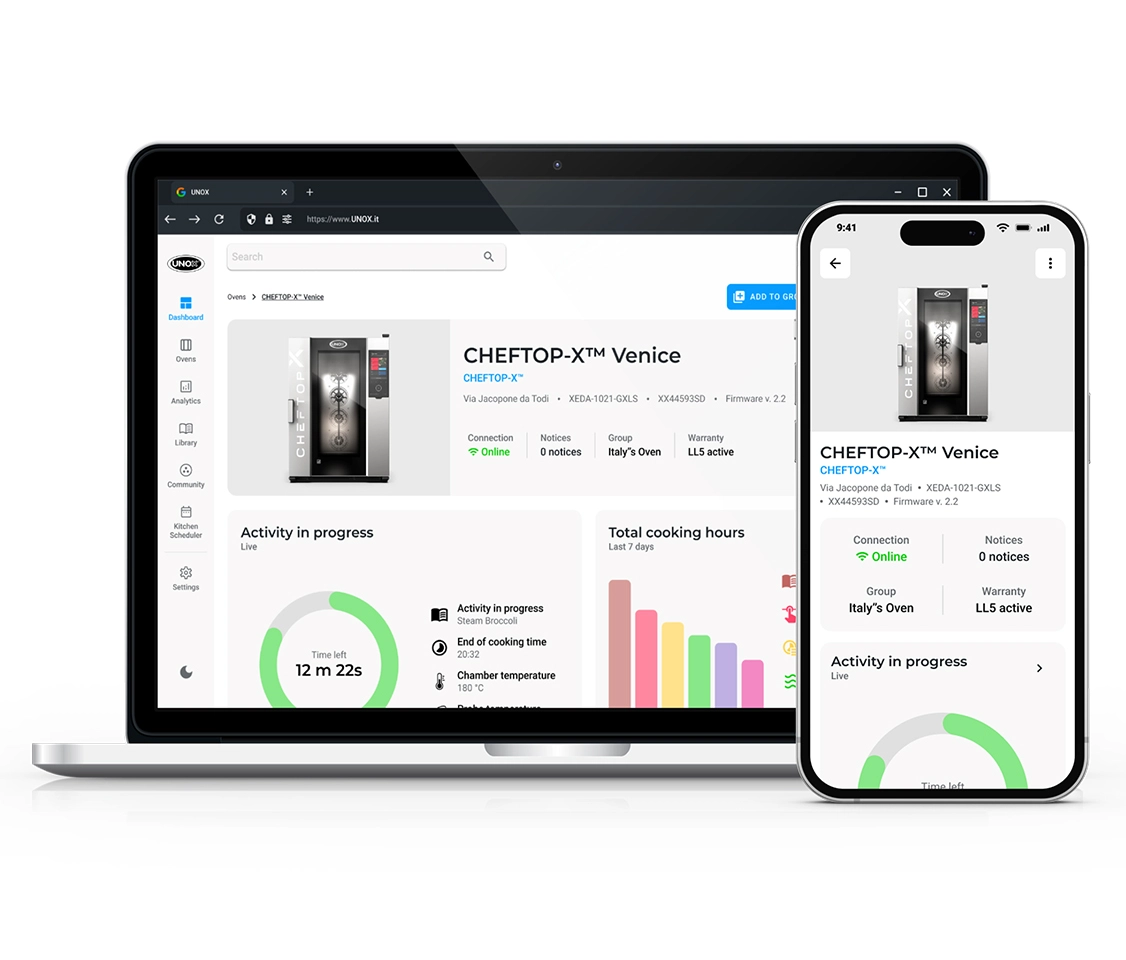
\includegraphics[alt={Immagine della applicazione \textit{DDC} su piattaforma \textit{Web e Mobile}}, height=10cm]{img/ddc.png}
    \caption{App \textit{DDC}: Applicazione \textit{DDC} su piattaforma \textit{Web} e Mobile}
    \label{fig:ddc}
\end{figure}


\section{Lo stage}
L'offerta di stage mi ha immediatamente intrigato per il suo focus su un progetto specifico vitale per l'azienda, piuttosto che un semplice esercizio accademico.
Questo aspetto ha richiesto un impegno significativo e una collaborazione intensa con diversi \textit{team} per portare a termine un progetto cruciale per l'azienda.
Nel contesto aziendale esistono due app chiamate \gls{ddc}\glox e \gls{ddcserviceg}\glox.
\begin{itemize}
    \item \textit{DDC} ha come utilizzatori i proprietari dei forni che utilizzano questa app per le funzionalità connesse dei loro dispositivi.
    \item \textit{DDC Service} ha come utilizzatori personale tecnico, personale responsabile di manutenzione dei forni e utenti addetti al \textit{Service}.
\end{itemize}
Per rispondere alle esigenze aziendali, è stato necessario avviare lo sviluppo di una nuova app \textit{DDC Service} con una prospettiva moderna e che sia multi-piattaforma.
Durante il mio stage presso \myAzienda, ho lavorato principalmente sull'avvio dello sviluppo di questa app, il mio obiettivo principale è stato ristrutturare e sviluppare completamente da zero \textit{DDC Service} precedentemente limitata alla piattaforma \textit{Web}.
Ho esteso le funzionalità di \textit{DDC Service} per renderla compatibile con dispositivi \textit{Android, iOS e Web}, integrando questa nuova versione nell'esistente \gls{monorepog}\glox di \textit{DDC}.
\\Questo approccio ha permesso di condividere il \gls{designsystemg}\glox e sfruttare l'infrastruttura esistente per ottimizzare l'efficienza e la manutenibilità del codice.
\\Durante il periodo di stage, ho collaborato attivamente con il \textit{team} di sviluppo, design e progettazione per implementare le prime funzionalità richieste per l'applicazione, rispettando le linee guida e assicurando la compatibilità su tutte le piattaforme \textit{target}.
Questa esperienza mi ha fornito competenze pratiche nello sviluppo software multi-piattaforma e una comprensione approfondita della progettazione scalabile e della gestione delle risorse tecniche in un ambiente \textit{monorepo}.


\newpage
    \chapter{Descrizione dello stage}
\label{chap:stage_descrizione}

\section{Pianificazione}
\subsection{Attività}
La seguente pianificazione delle attività è stata inizialmente delineata nel piano di lavoro. 
Tuttavia, durante lo stage, alcune attività sono state modificate sia per una maggiore comprensione emersa dall'analisi dei requisiti, sia per cambiamenti negli obiettivi da realizzare.
\subsubsection*{Prima Settimana (40 ore)}
\begin{itemize}
    \item Incontro con le persone coinvolte nel progetto per discutere i requisiti e le richieste relative al sistema da sviluppare.
    \item Verifica delle credenziali e degli strumenti di lavoro assegnati.
    \item Presa visione dell'infrastruttura esistente, in particolare della app \gls{ddc}\glox, del suo \gls{designsystemg}\glox e della \gls{monorepog}\glox esistente.
    \item Formazione sulle tecnologie adottate.
\end{itemize}

\subsubsection*{Seconda Settimana (40 ore)}
\begin{itemize}
    \item Studio del software \gls{backendg}\glox esistente con cui l'applicazione si integrerà.
    \item Avvio dello sviluppo dell'applicazione, definizione dell'architettura, dello \textit{stack} di navigazione e implementazione della funzionalità di autenticazione.
\end{itemize}

\subsubsection*{Terza Settimana (40 ore)}
\begin{itemize}
    \item Continuazione dello sviluppo dell'architettura dell'applicazione, inclusi il \textit{login} e lo \textit{stack} di navigazione principale.
\end{itemize}

\subsubsection*{Quarta Settimana (40 ore)}
\begin{itemize}
    \item Sviluppo della funzionalità consultazione Prodotto, detta \textit{Product Page}
\end{itemize}

\subsubsection*{Quinta Settimana (40 ore)}
\begin{itemize}
    \item Continuazione dello sviluppo delle funzionalità di consultazione Prodotto.
\end{itemize}

\subsubsection*{Sesta Settimana (40 ore)}
\begin{itemize}
    \item Implementazione nella \textit{Product Page} delle funzionalità di visualizzazione manuali, ricambistica e \textit{Tech and Docs} 
    \item Sviluppa della funzionalità consultazione \textit{Serviced Oven} 
\end{itemize}

\subsubsection*{Settima Settimana (40 ore)}
\begin{itemize}
    \item Sviluppo della funzionalità di gestione del flusso \gls{rma}\glox.
\end{itemize}

\subsubsection*{Ottava Settimana - Conclusione (40 ore)}
\begin{itemize}
    \item Continuazione dello sviluppo della funzionalità di gestione del flusso \textit{RMA}.
    \item Test e ottimizzazione dell'applicazione con il personale aziendale.
\end{itemize}

\begin{table}[ht]
    \centering
    \begin{tabular}{c|c}
    \hline\hline
    \textbf{Durata in ore} & \textbf{Descrizione dell'attività} \\
    \hline\hline
    40 & Inserimento in azienda \\
    \hline
    24 & Studio \textit{Backend} esistente \\
    \hline
    56 & Sviluppo architettura applicazione\\
    \hline
    80 & Sviluppo della funzionalità \textit{Product Page} \\
    \hline
    40 & Sviluppo della funzionalità \textit{Serviced Oven Page} \\
    \hline
    60 & Sviluppo funzionalità flusso \textit{RMA} \\
    \hline
    20 & Test e ottimizzazione della applicazione \\
    \hline
    \textbf{Totale ore} & \textbf{320} \\
    \hline\hline
    \end{tabular}
    \caption{Suddivisione delle ore di lavoro per le attività di progetto.}
    \label{tab:ore-lavoro}
    \end{table}

\subsection{Obbiettivi}
\subsubsection{Obiettivi obbligatori}
\begin{itemize}
    \item \textbf{Architettura dell'applicazione:} Definizione dello scheletro e dell'architettura dell'applicazione, compresa la navigazione.
    \item \textbf{Autenticazione: } Implementazione della funzionalità di autenticazione (\textit{SignIn, SignUp, Recover Password}).
    \item \textbf{\textit{Product Page}: }Sviluppo della funzionalità consultazione Prodotto e delle funzionalità di visualizzazione manuali, ricambistica e \textit{Tech and Docs}.
    \item \textbf{\textit{Serviced Oven}: }Sviluppa della funzionalità consultazione dei propri forni in \textit{service} detti \textit{Serviced Oven}.
    \item \textbf{Test piattaforme: } Esecuzione di test sulla piattaforma \textit{web} e \textit{mobile} per garantire la massima portabilità del codice.

\end{itemize}

\subsubsection{Obiettivi desiderabili}
\begin{itemize}
    \item \textbf{RMA:} Sviluppo della funzionalità di gestione del flusso \textit{RMA}.
\end{itemize}

\subsubsection{Obiettivi facoltativi}
\begin{itemize}
    \item \textbf{Test E2E:} Creazione di test automatizzati \gls{e2e}\glox per verificare le varie componenti dell'applicazione, per massimizzare l'efficienza del processo di \textit{testing}.
\end{itemize}

\subsection{Vincoli}

Durante lo sviluppo del progetto, sono stati identificati vari vincoli che hanno influenzato il contesto operativo e le decisioni progettuali. 
Questi vincoli hanno avuto un impatto significativo sulle scelte effettuate e sull'approccio adottato per la realizzazione dell'applicazione. 
I principali vincoli sono suddivisibili in categorie come vincoli aziendali, tecnologici, temporali e di design.
\subsubsection{Vincoli tecnologici}
Un vincolo importante riguardava l'adozione delle tecnologie già utilizzate da \myAzienda
L'applicazione doveva essere sviluppata utilizzando strumenti e tecnologie in uso all'interno dell'azienda per assicurare l'integrazione e la coerenza con l'ecosistema tecnologico esistente.
\subsubsection{Vincoli temporali}
Un vincolo temporale significativo era la data di conclusione dello stage, fissata per il 7 giugno 2024.
Questa scadenza ha imposto un termine rigido per il completamento del progetto, richiedendo una gestione attenta del tempo e delle risorse per rispettare il limite prestabilito.
\subsubsection{Vincoli di \textit{design}}
I vincoli di design includevano il rispetto del \gls{designsystemg}\glox aziendale e delle specifiche grafiche fornite dall'azienda.
L'applicazione doveva essere allineata al \textit{Design System} esistente e rispettare le palette di colori e le linee guida visive stabilite dall'azienda.

\section{Analisi preventiva dei rischi}
Durante la fase di analisi iniziale, sono stati individuati alcuni possibili rischi che avrebbero potuto causare problemi nel corso del progetto.
Per affrontarli, sono state elaborate delle possibili soluzioni.
\begin{risk}{Inesperienza tecnologica}
    \riskdescription{Era previsto l'utilizzo di tecnologie mai utilizzate prima, il che poteva causare rallentamenti nello sviluppo dell'applicazione}
    \risksolution{L'azienda ha programmato un periodo di circa una settimana dedicato allo studio autonomo delle tecnologie, utilizzando tutorial e risorse interne}
    \label{risk:inesperienza-tecnologica} 
\end{risk}

\begin{risk}{Difficoltà nel soddisfare le esigenze di \textit{design}}
    \riskdescription{Inizialmente era previsto realizzare le funzionalità richieste senza dare peso al \textit{design} e alla parte grafica dell'app.
    Tuttavia, è emersa la necessità di cooperare con il team di \textit{design} per seguire le loro linee guida}
    \risksolution{Si è utilizzato il \textit{Design System} già esistente, adattandolo dove necessario, e si è dato del tempo per imparare a utilizzare nuovi strumenti come Figma}
    \label{risk:design-system} 
\end{risk}

\begin{risk}{Interpretazione dei requisiti}
    \riskdescription{I requisiti avrebbero potuto subire aggiornamenti in corso d'opera a causa della difficoltà d'individuare con facilità se un requisito fosse realizzabile o meno}
    \risksolution{Sono stati pianificati \textit{meeting} regolari con i \textit{team} coinvolti per discutere e individuare soluzioni, semplificando la realizzazione dei requisiti proposti}
    \label{risk:interpretazione-requisiti} 
\end{risk}

\newpage
    \chapter{Tecnologie utilizzate}
\label{chap:tecnologie_utilizzate}
Questo capitolo esplora le tecnologie chiave adottate nel contesto dello sviluppo dell'applicazione \gls{ddcserviceg}\glox.
Vengono presentati i linguaggi di programmazione, i \textit{framework}, gli strumenti di sviluppo, le piattaforme di collaborazione e gestione, oltre alle soluzioni \textit{cloud} e \gls{devopsg}\glox impiegate per supportare e ottimizzare il processo di sviluppo.
Ogni tecnologia è discussa nel contesto del suo ruolo nell'ecosistema di sviluppo dell'applicazione, evidenziando come contribuisca alla scalabilità, alla manutenibilità e alla coerenza del codice, nonché al miglioramento complessivo dell'efficienza operativa dell'azienda.
\section{Linguaggi di programmazione}
\begin{itemize}
    \item \textbf{TypeScript}: è un linguaggio di programmazione \textit{open-source} sviluppato da Microsoft.
    TypeScript è un \textit{superset} di \textit{JavaScript} che aggiunge la tipizzazione statica opzionale e altre funzionalità moderne, rendendo il codice più robusto e manutenibile. 
    Questo linguaggio è stato utilizzato per lo sviluppo dell'applicazione \textit{DDC Service}, sia per la parte \gls{frontendg}\glox che per l'integrazione con i servizi \gls{backendg}\glox, garantendo una maggiore affidabilità e scalabilità del codice.
\end{itemize}

\section{\textit{Framework} in uso}
\begin{itemize}
    \item \textbf{Expo}: è un \textit{framework open-source} per la creazione di applicazioni \textit{React Native}.
    Facilita lo sviluppo di applicazioni \textit{mobile} fornendo strumenti e librerie preconfigurate.
    \textit{Expo} è stato utilizzato per lo sviluppo delle applicazioni \textit{Android} e \textit{IOS}, permettendo di scrivere il codice una sola volta e distribuirlo su entrambe le piattaforme in modo efficiente.
    \item \textbf{Next.js}: un \textit{framework} di sviluppo \textit{React} per la creazione di applicazioni \textit{Web}.
    Supporta il \textit{rendering} lato \textit{server} e la generazione di siti statici, migliorando così le prestazioni e l'ottimizzazione per i motori di ricerca (\textit{SEO}).
    \item \textbf{React}: è una libreria \textit{JavaScript} per la costruzione di interfacce utente sviluppata da \textit{Facebook}. React si distingue per la sua architettura basata su componenti e l'uso del \textit{virtual DOM}, che rendono lo sviluppo di interfacce utente reattive ed efficienti. In particolare, React è stato utilizzato come base per le applicazioni, consentendo la creazione di componenti riutilizzabili che migliorano la coerenza e la manutenibilità del codice.
    \item \textbf{React Native}: è un framework open-source per lo sviluppo di applicazioni mobili creato da \textit{Facebook}. React Native permette di utilizzare React e \textit{TypeScript} per costruire applicazioni native per \textit{iOS} e \textit{Android}. Unox utilizza React Native per sviluppare applicazioni mobili, permettendo al team di scrivere il codice una sola volta e distribuirlo su entrambe le piattaforme, semplificando e ottimizzando gli sforzi di sviluppo.
    \item \textbf{NodeJS}: è una piattaforma di \textit{runtime open-source} basata su \textit{JavaScript V8} di \textit{Chrome}, progettata per costruire applicazioni di rete veloci e scalabili. Unox utilizza NodeJS per l'esecuzione del codice \textit{TypeScript} e come gestore di pacchetti. Facilita le operazioni lato \textit{server}, consentendo una gestione efficiente di compiti come il \textit{rendering} del server e lo sviluppo di \textit{API}, migliorando le prestazioni e la scalabilità dell'applicazione.
\end{itemize}

\section{Tecnologie per \textit{monorepo}}
\begin{itemize}
\item \textbf{NPM Workspaces}: una funzionalità di NPM che consente di gestire più pacchetti all'interno di un unico \gls{repog}\glox.
\\\textit{NPM Workspaces} è stato utilizzato per organizzare i vari pacchetti del progetto \gls{ddcserviceg}\glox, semplificando la gestione delle dipendenze e migliorando l'efficienza dello sviluppo.
\item \textbf{NX}: un set di strumenti per la gestione di \gls{monorepog}\glox che facilita lo sviluppo, il test e la manutenzione di applicazioni e librerie su larga scala.
Nel progetto \textit{DDC Service}, NX è stato implementato nella parte finale per la gestione del \textit{monorepo}, per organizzare e gestire le dipendenze del codice e migliorando la modularità e la coerenza del progetto.
\end{itemize}

\section{Librerie utilizzate}
\begin{itemize}
    \item \textbf{Solito}: una libreria che permette di condividere il codice tra applicazioni \textit{Next} ed \textit{Expo}, riducendo la duplicazione del codice e semplificando la manutenzione.
    Nel contesto del progetto \gls{ddcserviceg}\glox, Solito è stato impiegato per ottimizzare la condivisione del codice tra le piattaforme web e mobile, implementando una gestione del routing comune tra le pagine.
    Ciò ha permesso di mantenere una struttura di navigazione coerente e una logica di gestione dei percorsi uniforme, migliorando l'esperienza dell'utente e semplificando lo sviluppo e la manutenzione dell'applicazione su entrambe le piattaforme.\footcite{site:solito}
    \item \textbf{Moti}: una libreria di animazioni per \textit{React Native}\glox che facilita la creazione di animazioni complesse e fluide.
    È stata utilizzata nel progetto \gls{ddcserviceg}\glox per migliorare l'interazione dell'utente e l'aspetto visivo delle applicazioni mobili.\footcite{site:moti}
    \item \textbf{Dripsy}: una libreria per la gestione dello stile di \textit{UI} per \textit{React Native} e \textit{Web}.
    Dripsy permette di definire uno stile una sola volta e applicarlo ovunque, supportando la creazione di interfacce responsive che si adattano automaticamente a diverse dimensioni di schermo. È compatibile con Expo, Vanilla React Native e Next.js, offrendo un supporto completo per TypeScript e facilitando l'implementazione di temi personalizzati e varianti di tema. Con una semplice \gls{api}\glox, è possibile definire stili tematici e responsivi in una sola riga di codice. Supporta anche modalità scura e personalizzazione dei colori.\footcite{site:dripsy}
    \item \textbf{Redux}: una libreria per la gestione dello stato delle applicazioni \textit{JavaScript}.
    \textit{Redux} è utilizzato per mantenere uno stato globale consistente e prevedibile nell'applicazione, facilitando la gestione dello stato complesso e la sincronizzazione dei dati tra i vari componenti.
    \item \textbf{Redux Toolkit (RTK)}: una serie di strumenti e convenzioni per semplificare l'uso di \textit{Redux}. \textit{RTK} include funzioni per la creazione di \textit{slice} di stato, \textit{middleware} personalizzati e la gestione di operazioni asincrone, rendendo lo sviluppo con \textit{Redux} più efficiente e meno soggetto a errori.
    \item \textbf{GraphQL}: un linguaggio di query per \textit{API}\glox.
    \textit{GraphQL} è utilizzato per ottenere dati in modo efficiente e flessibile, consentendo di specificare esattamente quali dati sono necessari.
    Nel progetto \gls{ddcserviceg}\glox, \textit{GraphQL} facilita la comunicazione tra il \gls{frontendg}\glox e il \gls{backendg}\glox, migliorando le performance e riducendo la quantità di dati trasferiti.
    \item \textbf{GraphQL Code Generator}: uno strumento per generare tipi \textit{TypeScript} per le query, le mutazioni e i frammenti definiti nello schema \textit{GraphQL}. Questo migliora la sicurezza del tipo e riduce gli errori di \textit{runtime}, mantenendo il codice sincronizzato con lo schema \textit{GraphQL}.
\end{itemize}


\section{Strumenti di sviluppo}
\begin{itemize}
\item \textbf{Visual Studio Code}: un \textit{editor} di codice sorgente sviluppato da \textit{Microsoft}, altamente estensibile e utilizzato per una varietà di linguaggi di programmazione.
\item \textbf{Xcode}: un ambiente di sviluppo integrato (\textit{IDE}) di \textit{Apple} per \textit{macOS}, utilizzato per sviluppare software per \textit{IOS}, \textit{macOS}, \textit{watchOS} e \textit{tvOS}.
\item \textbf{Android Studio}: un \textit{IDE} ufficiale per lo sviluppo di applicazioni \textit{Android}, fornito da \textit{Google}. Viene utilizzato per scrivere, eseguire il debug e testare le applicazioni \textit{Android}.
\item \textbf{Prettier}: uno strumento di formattazione del codice che aiuta a mantenere uno stile di codice coerente in tutti i progetti.
\item \textbf{Cocoapods}: un gestore di dipendenze per \textit{Swift} e \textit{Objective-C Cocoa projects}. Viene utilizzato per integrare librerie di terze parti nei progetti \textit{iOS}.
\end{itemize}

\section{Piattaforme di collaborazione e gestione}
\begin{itemize}
\item \textbf{Git}: viene utilizzato come sistema di controllo delle versioni per il tracciamento delle modifiche al codice sorgente.
\item \textbf{Microsoft Teams}: adottato come strumento di comunicazione e collaborazione in tempo reale all'interno dell'azienda, facilitando le discussioni, le videochiamate e la condivisione di documenti. Viene utilizzato anche per la calendarizzazione di eventi e meeting.
\end{itemize}

\section{Piattaforme \textit{cloud} e \textit{DevOps}}
\begin{itemize}
\item \textbf{Microsoft Azure}: una piattaforma cloud utilizzata per l'hosting di applicazioni, servizi e dati aziendali. Viene utilizzato da Unox per l'hosting di alcuni dei servizi principali. Dalla suite di Azure, viene utilizzato anche \textit{Azure DevOps} per la gestione delle attività di sviluppo software, tra cui la gestione dei repository Git, delle build e delle attività.
\item \textbf{AWS}: \textit{Amazon Web Services} (\textit{AWS}) è un altro servizio cloud utilizzato per le risorse di calcolo, archiviazione e servizi di rete. Alcuni dei servizi secondari di Unox sono ospitati su AWS.
\item \textbf{Amplify}: è una piattaforma di sviluppo di applicazioni cloud che facilita l'integrazione di funzionalità come autenticazione, \textit{API}, \textit{storage} e altro ancora.
In questo progetto, \textit{Amplify} è stato utilizzato per scaricare automaticamente le chiavi di accesso, migliorando la sicurezza e semplificando la gestione delle credenziali.
Inoltre, Amplify è stato impiegato per implementare le notifiche \textit{push}, permettendo una comunicazione efficace e tempestiva con gli utenti dell'applicazione.
\end{itemize}

\section{Strumenti di \textit{design}}
\begin{itemize}
\item \textbf{Figma}: uno strumento di design collaborativo utilizzato per la progettazione delle interfacce utente. Facilita la collaborazione tra \textit{designer} e sviluppatori e permette di creare e condividere facilmente prototipi e \textit{design}.
\end{itemize}


\newpage
    \chapter{Analisi dei requisiti}
\label{chap:analisi_requisiti}

\section{Caratteristiche del utente}
Per esaminare la \textit{user base} dell'app \gls{ddcserviceg}\glox bisogna tenere in considerazione 
che tutti i dati di cui l'applicazione fa uso saranno reperibili dal \gls{backendg}\glox associato all'applicazione.
Le basi di dati con cui il \textit{backend} andrà a comunicare saranno popolate da piattaforme esterne ignote alla app in questione.
Il sistema di autenticazione non dovrà tenere in considerazione di tipologie di utenti speciali come \textit{Admin} o \textit{SysAdmin}.

Questi utenti possono far parte del personale Unox oppure possono essere professionisti con cui Unox collabora.
Sono persone che richiedono di accedere alla app sia da \textit{Desktop} tramite \textit{web-app} mentre sono in ufficio, che da \textit{app} sul proprio \textit{smartphone} mentre sono in mobilità.
La user base della app è composta da personale tecnico, personale responsabile alla vendita e utenti addetti al \textit{Service}.
Non esiste però la necessità lato autenticazione di rendere il processo di registrazione o di \textit{login} diverso in base alla funzione del utente o in base alla sua appartenenza.
In linea generica tutti gli utenti registrati hanno gli stessi permessi.
In futuro l'applicazione necessiterà di un sistema per rendere un utente registrato verificato o meno, però per questo progetto questa richiesta non è una necessità.

\section{Vincoli generali}
Date le premesse sulle caratteristiche degli utenti della applicazione, definiremo quindi solo due categorie di utenti: Utente Autenticato, Utente Non Autenticato.
Ho individuato i seguenti attori:
\begin{description}
	\item[Utente Non Autenticato] L'Utente Non Autenticato è una tipologia di utente che o non si è ancora registrato e quindi non possiede delle credenziali oppure possiede delle credenziali ma deve ancora far il processo di \textit{login} detto \textit{sign in}.
	\item[Utente Autenticato] L'Utente Autenticato è una tipologia di utente che possiede delle credenziali valide e che ha completato con successo il processo di \textit{login} detto \textit{sign in}.
\end{description}

\section{Casi d'uso}
I seguenti casi d'uso sono state formulati solo per le funzionalità che sono state realmente realizzate in quanto le funzionalità opzionali per le quali non si ha avuto tempo non sono state tenute in considerazione per l'analisi dei requisiti.

\begin{usecase}{0}{Autenticazione}
    \usecaseactors{Utente Non Autenticato}
    \usecasepre{Un Utente Non Autenticato vuole accedere alle funzionalità della \textit{app}}
    \usecasedesc{Questo scenario descrive un utente che vuole accedere alla funzionalità della \textit{app} ma che non ne ha i permessi, per tanto deve fare la registrazione (\textit{sing up}) o il \textit{login} (\textit{sign in})}
    \usecasepost{l'utente accede al processo di registrazione o di \textit{login}}
    \label{uc:uc_scenario_autenticazione}
\end{usecase}

\begin{usecase}{0.1}{Registrazione}
    \usecaseactors{Utente Non Autenticato}
    \usecasepre{Un Utente Non Autenticato NON possiede delle credenziali per poter accedere alla \textit{app}.}
    \usecasedesc{Questo scenario descrive un utente che non possiede credenziali di autenticazione e che non riesce ad accedere alle funzionalità della \textit{app}, per tanto intraprende il processo di registrazione con cui alla fine riuscirà ad avere delle credenziali valide.}
    \usecasepost{L'utente ora ha delle credenziali valide con cui poter effettuare il \textit{login} e diventare un Utente Autenticato}
    \usecasealt{Se l'utente non fornisce con correttezza tutti i dati necessari alla registrazione, visualizza un messaggio di errore.}
    \label{uc:uc_scenario_autenticazione_reg}
\end{usecase}

\begin{usecase}{0.2}{Login}
    \usecaseactors{Utente Non Autenticato}
    \usecasepre{Un Utente non Autenticato che possiede delle credenziali valide per l'autenticazione.}
    \usecasedesc{Tramite questo scenario l'utente fornisce le sue credenziali per l'autenticazione e completa il processo di \textit{login}.}
    \usecasepost{L'utente è diventato un Utente Autenticato}
    \usecasealt{Se l'utente fornisce delle credenziali sbagliate, visualizza un messaggio di errore.}
    \label{uc:uc_scenario_autenticazione_login}
\end{usecase}

\begin{usecase}{0.3}{Recover Password}
    \usecaseactors{Utente Non Autenticato}
    \usecasepre{Un Utente non Autenticato che possiede delle credenziali NON valide per l'autenticazione.}
    \usecasedesc{Tramite questo scenario l'utente fornisce le sue credenziali in maniera parziale e tramite un processo riesce a ripristinarle per poter avere delle credenziali valide.}
    \usecasepost{L'utente ha delle credenziali valide.}
    \label{uc:uc_scenario_autenticazione_recover}
\end{usecase}
\pagebreak
\begin{usecase}{1}{Visualizzazione Prodotto}
    \usecaseactors{Utente Autenticato}
    \usecasepre{Un utente ha completato con successo il processo di autenticazione.}
    \usecasedesc{L'utente visualizza le informazioni di un determinato prodotto incluse le sue parti commerciali e i dettagli tecnici a lui associati.}
    \usecasepost{L'utente ha visualizzato le informazioni collegate al prodotto richiesto.}
    \usecasealt{Se il prodotto richiesto non è esistente, viene visualizzato un messaggio di errore.}
    \label{uc:uc_scenario_prodotto}
\end{usecase}

\begin{usecase}{2}{Visualizzazione Serviced Oven}
    \usecaseactors{Utente Autenticato}
    \usecasepre{Un utente ha completato con successo il processo di autenticazione e ha tra i suoi forni alcuni dispositivi categorizzati come  \textit{Serviced Oven}, cioè forni a cui l'utente presta assistenza o manutenzione.}
    \usecasedesc{L'utente visualizza le informazioni di un determinato \gls{servicedoveng}\glox di cui ne ha i permessi.}
    \usecasepost{L'utente ha visualizzato le informazioni collegate al \textit{Serviced Oven} richiesto.}
    \usecasealt{Se il prodotto richiesto non è esistente, viene visualizzato un messaggio di errore.}
    \label{uc:uc_scenario_servicedoven}
\end{usecase}

\pagebreak
\section{Tracciamento dei requisiti}
Da un'attenta analisi dei requisiti e degli \textit{use case} effettuata sul progetto è stata stilata la tabella che traccia i requisiti in rapporto agli \textit{use case}.\\
Sono stati individuati diversi tipi di requisiti e si è quindi fatto utilizzo di un codice identificativo per distinguerli.\\
Il codice dei requisiti, dove ogni requisito è identificato con il carattere \textbf{R}, è così strutturato:
\begin{enumerate}
    \item[\textbf{F}:] Funzionale.
    \item[\textbf{Q}:] Qualitativo.
    \item[\textbf{V}:] Di vincolo.
    \item[\textbf{N}:] Obbligatorio (necessario).
    \item[\textbf{D}:] Desiderabile.
\end{enumerate}

Nelle tabelle \ref{tab:requisiti_funzionali}, \ref{tab:requisiti_qualitativi} e \ref{tab:requisiti_vincolo} sono riassunti i requisiti e il loro tracciamento con gli use case delineati in fase di analisi.

\section{Tabelle dei requisiti}


\begin{center}
    \rowcolors{1}{}{tableGray}
    \begin{longtable}{|p{2.25cm}|p{7.75cm}|p{2.25cm}|}
    \hline
    %\rowcolor{hyperColor!5}
    \multicolumn{1}{|c|}{\textbf{Requisito}} & \multicolumn{1}{c|}{\textbf{Descrizione}} & \multicolumn{1}{c|}{\textbf{Use Case}}\\
    \hline 
    \endfirsthead
    \rowcolor{white}
    \multicolumn{3}{c}{{\bfseries \tablename\ \thetable{} -- Continuo della tabella}}\\
    \hline
    %\rowcolor{hyperColor!5}
    \multicolumn{1}{|c|}{\textbf{Requisito}} & \multicolumn{1}{c|}{\textbf{Descrizione}} & \multicolumn{1}{c|}{\textbf{Use Case}}\\
    \hline 
    \endhead
    \hline
    \rowcolor{white}
    \multicolumn{3}{|r|}{{Continua nella prossima pagina...}}\\
    \hline
    %\caption{Tabella del tracciamento dei requisiti qualitativi.}
    \endfoot
    \endlastfoot
    RFN-1 & La funzionalità di autenticazione deve essere accessibile solo a Utenti Non Autenticati & UC0 \\
    \hline
    RFN-2 & L'utente deve essere in grado di accedere alla pagina registrazione detta \textit{sign up}. Questa pagina deve dare la possibilità di inserire i campi \textit{Name, Surname, Email, Password, Confirm Password, Company Name, Business Type, Address, Phone Number, Contry, Language} e scelte \textit{checkbox} GDPR e consenso Marketing & UC0.1 \\
    \hline
    RFN-2.1 & Nel \textit{form} per la registrazione devono esserci filtri per il controllo dei dati immessi come \textit{input} & UC0.1 \\
    \hline
    RFN-2.2 & Una volta immessi i dati nel \textit{form} della pagina di registrazione questa deve mostrare un messaggio che indica al utente di attivare l'account con la conferma della \textit{email} & UC0.1 \\
    \hline
    RFD-2.2.1 & Una volta confermata la email il processo di registrazione è completato, è richiesto che la app faccia automaticamente il \textit{login} con l'account appena creato, quindi ad ogni registrazione avviene il \textit{login} automatico & UC0.1 \\
    \hline
    RFN-3 & Nella pagina di \textit{login} l'utente presenta le sue credenziali nel apposito \textit{form}, cioè \textit{email e password} per poter diventare un Utente Autenticato & UC0.2 \\
    \hline
    RFN-3.1 & Nella pagina di \textit{login} nel caso in cui l'utente abbia inserito le credenziali non valide deve apparire un messaggio di errore & UC0.2 \\
    \hline
    RFN-4 & Deve esistere una pagina collegata alla pagina di \textit{login} che permetta di fare il processo di ripristino \textit{password}, detto \textit{Recover Password}, con questo processo l'utente inserisce la propria \textit{email} e dopo un processo di verifica gli viene confermato il ripristino della \textit{password} & UC0.3 \\
    \hline
    RFN-5 & La funzionalità di Prodotti definisce la \textit{feature} di visualizzazione di prodotti di Unox, sono tutti i prodotti esistenti e sono oggetti astratti da catalogo, non macchine reali, è richiesto solo la visualizzazione di un singolo prodotto nella sua \textit{Product Page} & UC1 \\
    \hline
    RFN-5.1 & Un prodotto deve essere identificato dal proprio \gls{productcodeg}\glox, se lo si identifica solo con il \textit{product code} si intende che si vuole visualizzare il prodotto con l'ultimo \gls{ecng}\glox & UC1 \\
    \hline
    RFN-5.2 & Nel caso in cui si identifichi un prodotto tramite il suo seriale, si intende che si vuole una istanza di un prodotto, quindi un prodotto fisico realmente esistente. Questa metodologia permette di identificare un prodotto con un \textit{ecng} specifico.& UC1 \\
    \hline
    RFN-5.3 & Nella pagina visualizzazione prodotto deve essere possibile visualizzare informazioni riguardanti le specifiche del prodotto, i documenti al prodotto collegati ed i \textit{files} scaricabili come \gls{firmwareg}\glox o modelli 3D.& UC1 \\
    \hline
    RFN-6 & Deve essere implementata la \textit{feature} Service, in particolare \gls{servicedoveng}\glox, è richiesto che l'utente visualizzi un singolo suo prodotto identificato con un seriale& UC2 \\
    \hline
    RFN-6.1 & Nella pagina di \textit{Serviced Oven} si devono poter visualizzare le informazioni riguardanti la connessione, si deve poter avere riferimenti alla pagina Prodotto del forno, e poter visualizzare e modificare le informazioni aggiuntive legate al prodotto, in particolare informazioni legate al cliente presso cui il forno è installato.& UC2 \\
    \hline
    RFN-7 & Per tutte le piattaforme deve essere realizzato un sistema di navigazione che permetta di cambiare le sezioni della app & UC0, UC1, UC2 \\
    \hline
    RFN-7.1 & Per le piattaforme \textit{mobile} è prevista la realizzazione di una \gls{tabbarg}\glox invece per la piattaforma \textit{web} è prevista la realizzazione di una \gls{navbarg}\glox & UC0, UC1, UC2 \\
    \hline
    \hiderowcolors
    \caption{Tabella del tracciamento dei requisiti funzionali.}
    \label{tab:requisiti_funzionali}
    \end{longtable}
\end{center}

\begin{center}
    \rowcolors{1}{}{tableGray}
    \begin{longtable}{|p{2.25cm}|p{7.75cm}|p{2.25cm}|}
    \hline
    %\rowcolor{hyperColor!5}
    \multicolumn{1}{|c|}{\textbf{Requisito}} & \multicolumn{1}{c|}{\textbf{Descrizione}} & \multicolumn{1}{c|}{\textbf{Use Case}}\\
    \hline 
    \endfirsthead
    \rowcolor{white}
    \multicolumn{3}{c}{{\bfseries \tablename\ \thetable{} -- Continuo della tabella}}\\
    \hline
    %\rowcolor{hyperColor!5}
    \multicolumn{1}{|c|}{\textbf{Requisito}} & \multicolumn{1}{c|}{\textbf{Descrizione}} & \multicolumn{1}{c|}{\textbf{Use Case}}\\
    \hline 
    \endhead
    \hline
    \rowcolor{white}
    \multicolumn{3}{|r|}{{Continua nella prossima pagina...}}\\
    \hline
    %\caption{Tabella del tracciamento dei requisiti qualitativi.}
    \endfoot
    \endlastfoot
    RQN-1 & La navigazione della app deve essere funzionale sia da \textit{mobile} che da \textit{web}, permettendo di indentificare con facilità il corretto flusso di funzionamento della \textit{app} indipendentemente dalla piattaforma in uso. & - \\
    \hline
    RQN-2 & Il codice prodotto deve essere scalabile e mantenibile, rispettando i \textit{design pattern} attualmente già utilizzati nel ecosistema Unox. & - \\
    \hline
    RQN-3 & Tutte le funzionalità realizzate devono essere testate su tutte le piattaforme di destinazione garantendo il loro funzionamento. & - \\
    \hline
    \hiderowcolors
    \caption{Tabella del tracciamento dei requisiti qualitativi.}
    \label{tab:requisiti_qualitativi}
    \end{longtable}
\end{center}

\begin{center}
    \rowcolors{1}{}{tableGray}
    \begin{longtable}{|p{2.25cm}|p{7.75cm}|p{2.25cm}|}
    \hline
    %\rowcolor{hyperColor!5}
    \multicolumn{1}{|c|}{\textbf{Requisito}} & \multicolumn{1}{c|}{\textbf{Descrizione}} & \multicolumn{1}{c|}{\textbf{Use Case}}\\
    \hline 
    \endfirsthead
    \rowcolor{white}
    \multicolumn{3}{c}{{\bfseries \tablename\ \thetable{} -- Continuo della tabella}}\\
    \hline
    %\rowcolor{hyperColor!5}
    \multicolumn{1}{|c|}{\textbf{Requisito}} & \multicolumn{1}{c|}{\textbf{Descrizione}} & \multicolumn{1}{c|}{\textbf{Use Case}}\\
    \hline 
    \endhead
    \hline
    \rowcolor{white}
    \multicolumn{3}{|r|}{{Continua nella prossima pagina...}}\\
    \hline
    \endfoot
    \endlastfoot
    
    RVN-1 & Le pagine e i componenti della applicazione devono essere realizzati tenendo conto delle indicazioni date dal \textit{team} di \textit{Design}, rispettando un \gls{designsystemg}\glox esistente e le convenzioni date per stili grafici compresi \textit{UI/UX} & - \\
    \hline
    RVN-2 & Le \textit{feature} realizzate per la applicazione devono essere compatibili con tutte le piattaforme di destinazione. & - \\
    \hline
    \hiderowcolors
    \caption{Tabella del tracciamento dei requisiti di vincolo.}
    \label{tab:requisiti_vincolo}
    \end{longtable}
\end{center}

\newpage



    \chapter{Progettazione e codifica}
\label{chap:design_coding}
Breve introduzione al capitolo

\section{Tecnologie e strumenti}
\label{sec:tecnologie-strumenti}
Di seguito viene data una panoramica delle tecnologie e strumenti utilizzati.

\subsection*{Tecnologia 1}
Descrizione Tecnologia 1.

\section{Ciclo di vita del software}
\label{sec:ciclo-vita-software}

\section{Progettazione}
\label{sec:progettazione}



\newpage
    \chapter{Studio fattibilità app in monorepo}
\label{chap:analisi-requisiti}

\section{Descrizione della monorepo}

\section{Descrizione routing e navigazione}

\section{Problemi riscontrati}

\subsection{Versionamento dipendenze}

\subsection{Isolamento delle dipendenze}


\newpage
    \chapter{Conclusioni}
\label{chap:conclusioni}
\section{Consuntivo finale}

L'attività di \textit{stage} ha seguito un piano di lavoro ben definito con obiettivi chiari.
Tutte le attività svolte hanno dato un esito positivo e hanno dato un prodotto più che sufficiente.
Durante il periodo di stage, ci sono stati momenti di difficoltà che hanno rallentato lo sviluppo.
Le principali problematiche incontrate sono state legate alla gestione della \gls{monorepog}\glox e all'implementazione dell'autenticazione nel \gls{backendg}\glox.
Ritengo che questo periodo sia stato molto utile sia per me che per l'azienda, poiché tutto il lavoro svolto ha contribuito a migliorare la gestione di queste problematiche per il futuro.
Ho collaborato attivamente con i membri del \textit{team} Unox e ogni momento di difficoltà è diventato un'opportunità di discussione costruttiva.
L'obiettivo non era solo risolvere i problemi, ma anche comprenderli e prevenire simili situazioni in futuro.
Lo sviluppo delle pagine richieste è stato valutato positivamente dall'azienda.
Di seguito sono riepilogati gli obiettivi e i requisiti raggiunti:

\pagebreak
\subsection{Requisiti raggiunti}


\begin{center}
    \rowcolors{1}{}{tableGray}
    \begin{longtable}{|p{2.25cm}|p{5cm}|}
    \hline
    \multicolumn{1}{|c|}{\textbf{Identificatore}} & \multicolumn{1}{c|}{\textbf{Soddisfatto/non}} \\
    \hline 
    \endfirsthead
    \rowcolor{white}
    \multicolumn{2}{c}{{\bfseries \tablename\ \thetable{} -- Continuazione}}\\
    \hline
    \multicolumn{1}{|c|}{\textbf{Identificatore}} & \multicolumn{1}{c|}{\textbf{Soddisfatto/non}} \\
    \hline 
    \endhead
    \hline
    \rowcolor{white}
    \multicolumn{2}{|r|}{{Continua nella prossima pagina...}}\\
    \hline
    \endfoot
    \endlastfoot
    
    RFN-1 & Soddisfatto  \\
    RFN-2 & Soddisfatto  \\
    RFN-2.1 & Soddisfatto  \\
    RFN-2.2 & Soddisfatto  \\
    RFD-2.2.1 & Soddisfatto  \\
    RFN-3 & Soddisfatto  \\
    RFN-3.1 & Soddisfatto  \\
    RFN-4 & Soddisfatto  \\
    RFN-5 & Soddisfatto  \\
    RFN-5.1 & Soddisfatto  \\
    RFN-5.2 & Soddisfatto  \\
    RFN-5.3 & Soddisfatto  \\
    RFN-6 & Soddisfatto  \\
    RFN-6.1 & Soddisfatto  \\
    RFN-7 & Soddisfatto  \\
    RFN-7.1 & Soddisfatto  \\
    RQN-1 & Soddisfatto  \\
    RQN-2 & Soddisfatto  \\
    RVN-1 & Soddisfatto  \\
    RVN-2 & Soddisfatto  \\
    \hline

    \hiderowcolors
    \caption{Tabella dei requisiti soddisfatti.}
    \label{tab:requisiti_soddisfatti}
    \end{longtable}
\end{center}

Come si può vedere dalla tabella sopra tutti i requisiti sono stati soddisfatti.
Il piano di lavoro è stato modificato nel momento in cui si è fatta l'analisi dei requisiti.
Fin dall'inizio sono stati delineati requisiti specifici dettagliandoli solo per gli obiettivi realizzabili.

\pagebreak
\subsection{Raggiungimento degli obiettivi}

\begin{center}
    \rowcolors{1}{}{tableGray}
    \begin{longtable}{|p{5cm}|p{2.75cm}|p{4cm}|}
    \hline
    \multicolumn{1}{|c|}{\textbf{Obiettivo}} & \multicolumn{1}{c|}{\textbf{Tipologia}} & \multicolumn{1}{c|}{\textbf{Raggiunto/non}} \\
    \hline 
    \endfirsthead
    \rowcolor{white}
    \multicolumn{3}{c}{{\bfseries \tablename\ \thetable{} -- Continuazione}}\\
    \hline
    \multicolumn{1}{|c|}{\textbf{Obiettivo}} & \multicolumn{1}{c|}{\textbf{Tipologia}} & \multicolumn{1}{c|}{\textbf{Raggiunto/non}} \\
    \hline 
    \endhead
    \hline
    \rowcolor{white}
    \multicolumn{3}{|r|}{{Continua nella prossima pagina...}}\\
    \hline
    \endfoot
    \endlastfoot
    
    Architettura dell'applicazione & Obbligatorio & Raggiunto  \\
    Autenticazione & Obbligatorio & Raggiunto  \\
    Product Page & Obbligatorio & Raggiunto  \\
    Serviced Oven & Obbligatorio & Raggiunto  \\
    Test piattaforme & Obbligatorio & Raggiunto  \\
    RMA & Desiderabile & Non Raggiunto  \\
    Test E2E & Facoltativo & Non Raggiunto  \\
    \hline

    \hiderowcolors
    \caption{Tabella degli obiettivi raggiunti.}
    \label{tab:obiettivi_raggiunti}
    \end{longtable}
\end{center}
Quasi tutti gli obiettivi di sviluppo dello \textit{stage} sono stati raggiunti. Il flusso di lavoro dei \gls{rmag}\glox non è stato avviato in quanto avrebbe richiesto troppo tempo, e si è deciso di dedicare le risorse ad attività con maggiore priorità. L'obiettivo dei test \gls{e2eg}\glox, proposto da me per il progetto, è stato riconosciuto come utile.
Fin dall'inizio, ho ritenuto importante trovare una metodologia pratica per realizzare test \textit{E2E} integrabili nella \gls{cicdg}\glox e che siano multipiattaforma.
Anche in questo caso, si è deciso di concentrare gli sforzi su attività più rilevanti.

Il resto degli obiettivi sono stati raggiunti con successo, permettendo di consegnare un prodotto utilizzabile dall'azienda e conforme alle loro richieste.

\section{Applicazione consegnata}

È stata consegnata l'applicazione \gls{ddcserviceg}\glox funzionante e disponibile in \textit{development} su \textit{iOS}, \textit{Android} e \textit{web}.
Tra le pagine e le funzionalità realizzate, vorrei evidenziare le seguenti:

\begin{figure}[H]
    \centering
    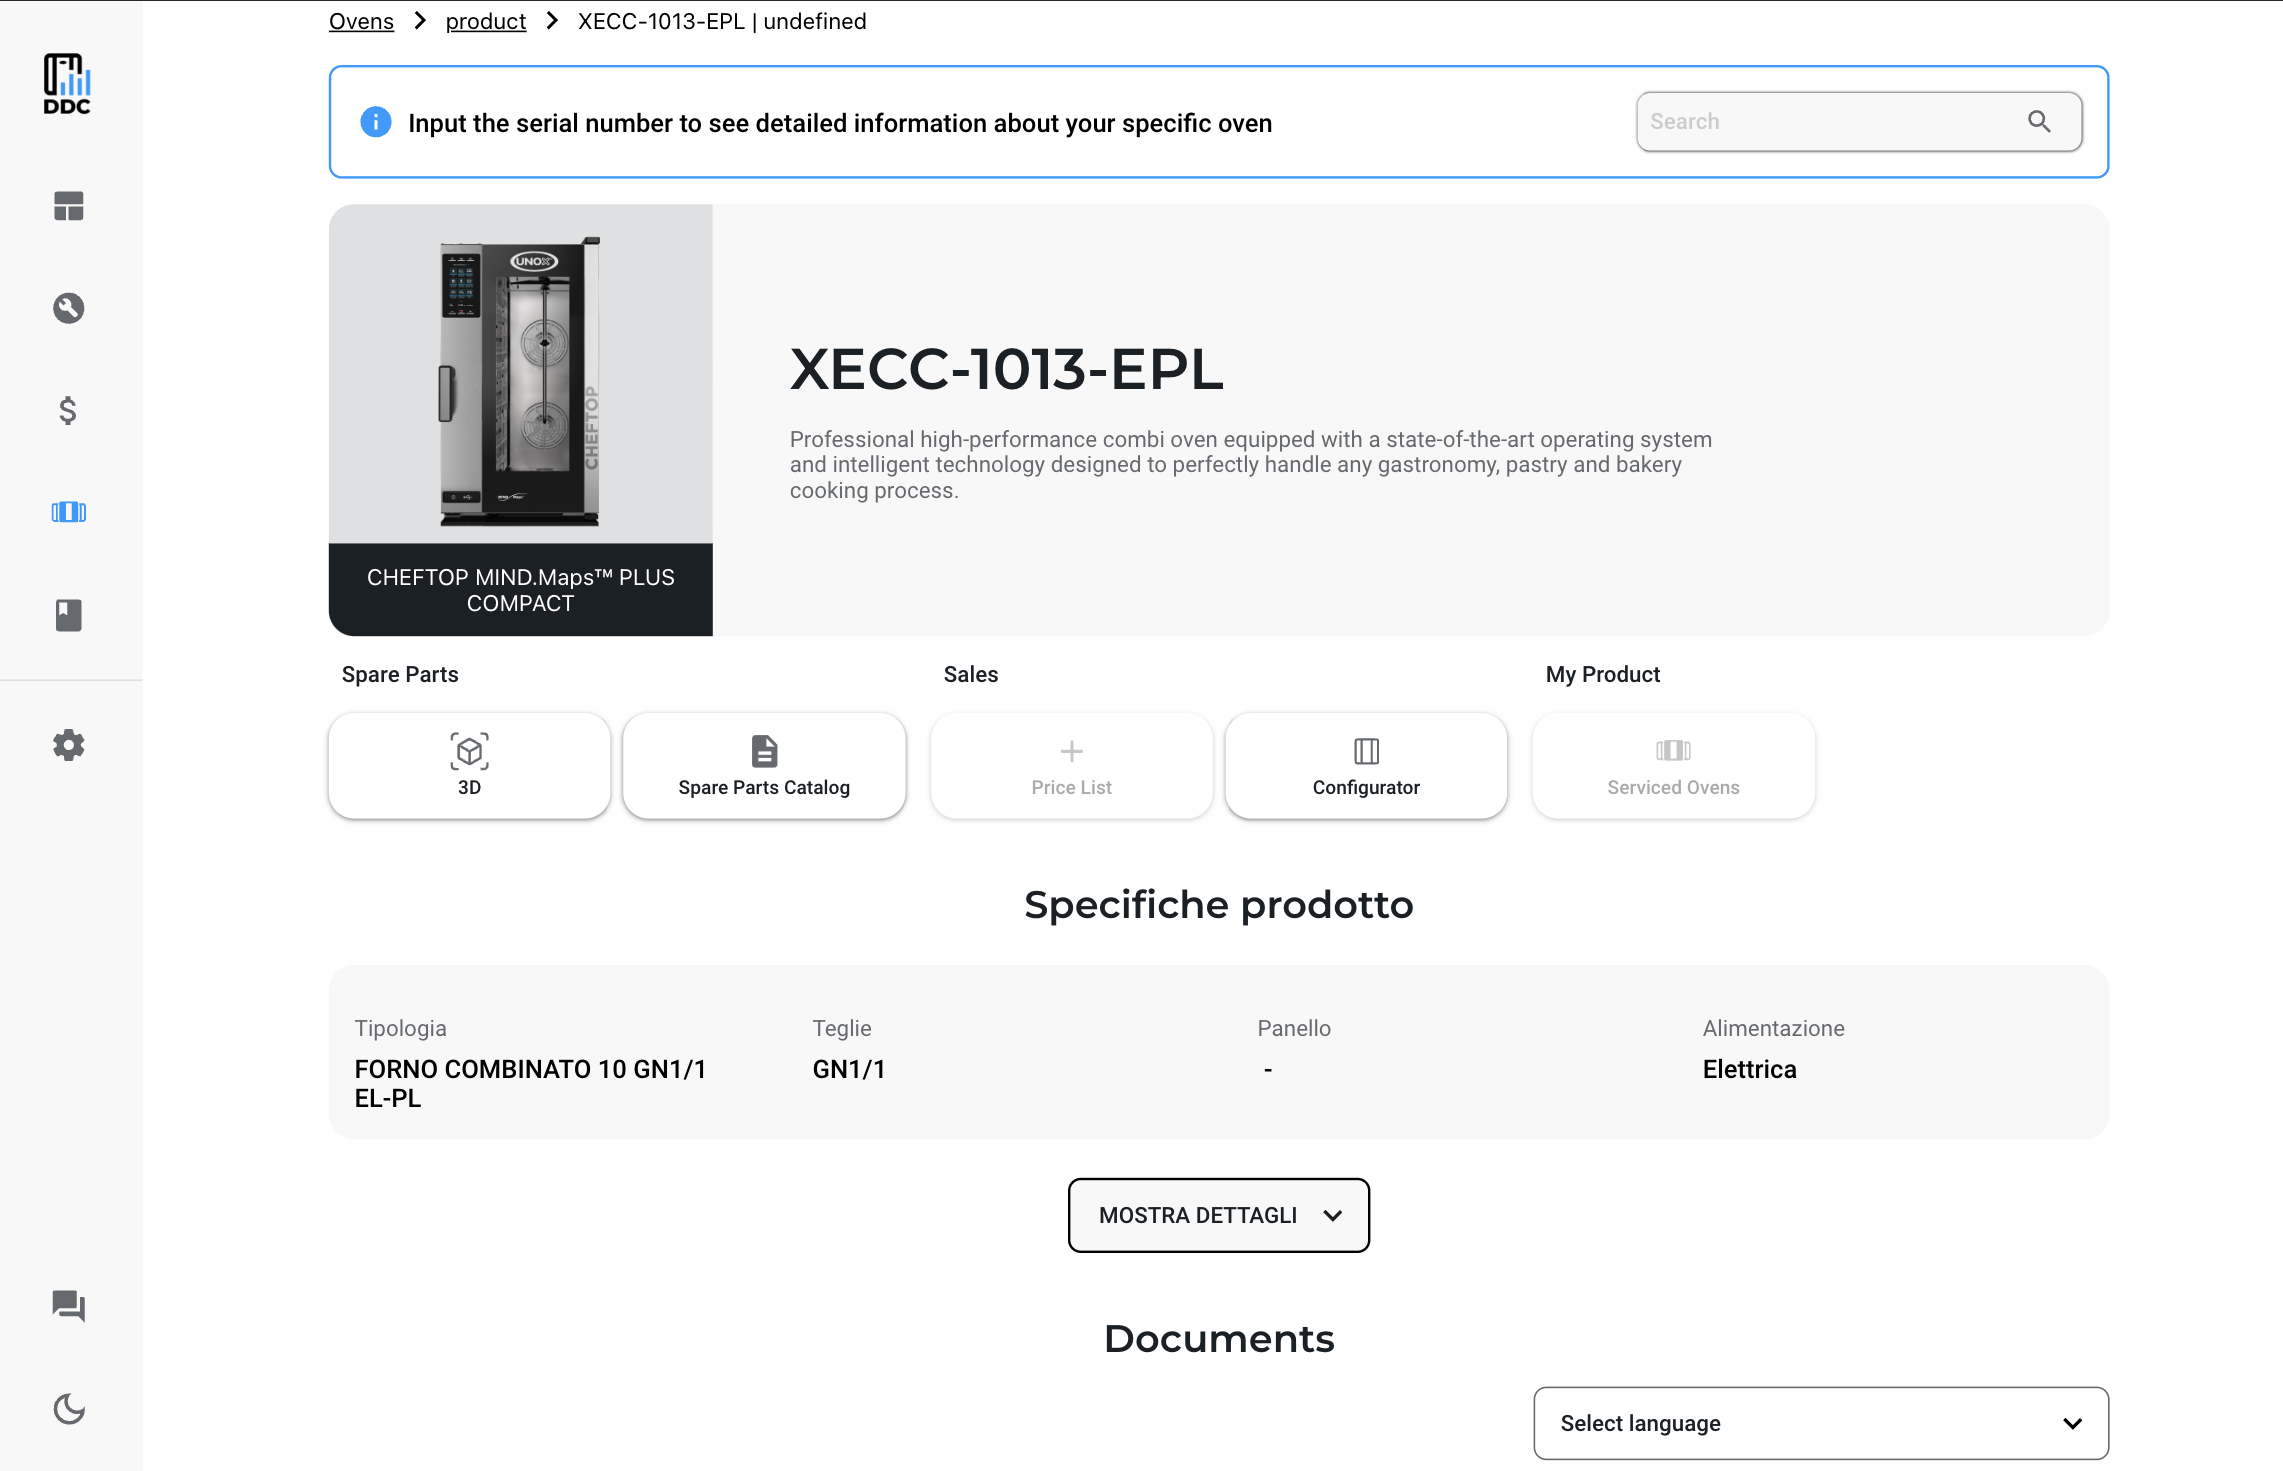
\includegraphics[alt={Screenshot della pagina \textit{"Product Page"} su piattaforma \textit{web}}, height=10cm]{img/ProductPageWeb}
    \caption{App \textit{DDC Service} pagina \textit{Product Page} piattaforma \textit{Web}}
    \label{fig:productpageweb}
\end{figure}

La figura mostra la pagina \textit{"Product Page"} della piattaforma \textit{web} dell'applicazione \textit{DDC Service}.

\begin{figure}[H]
    \centering
    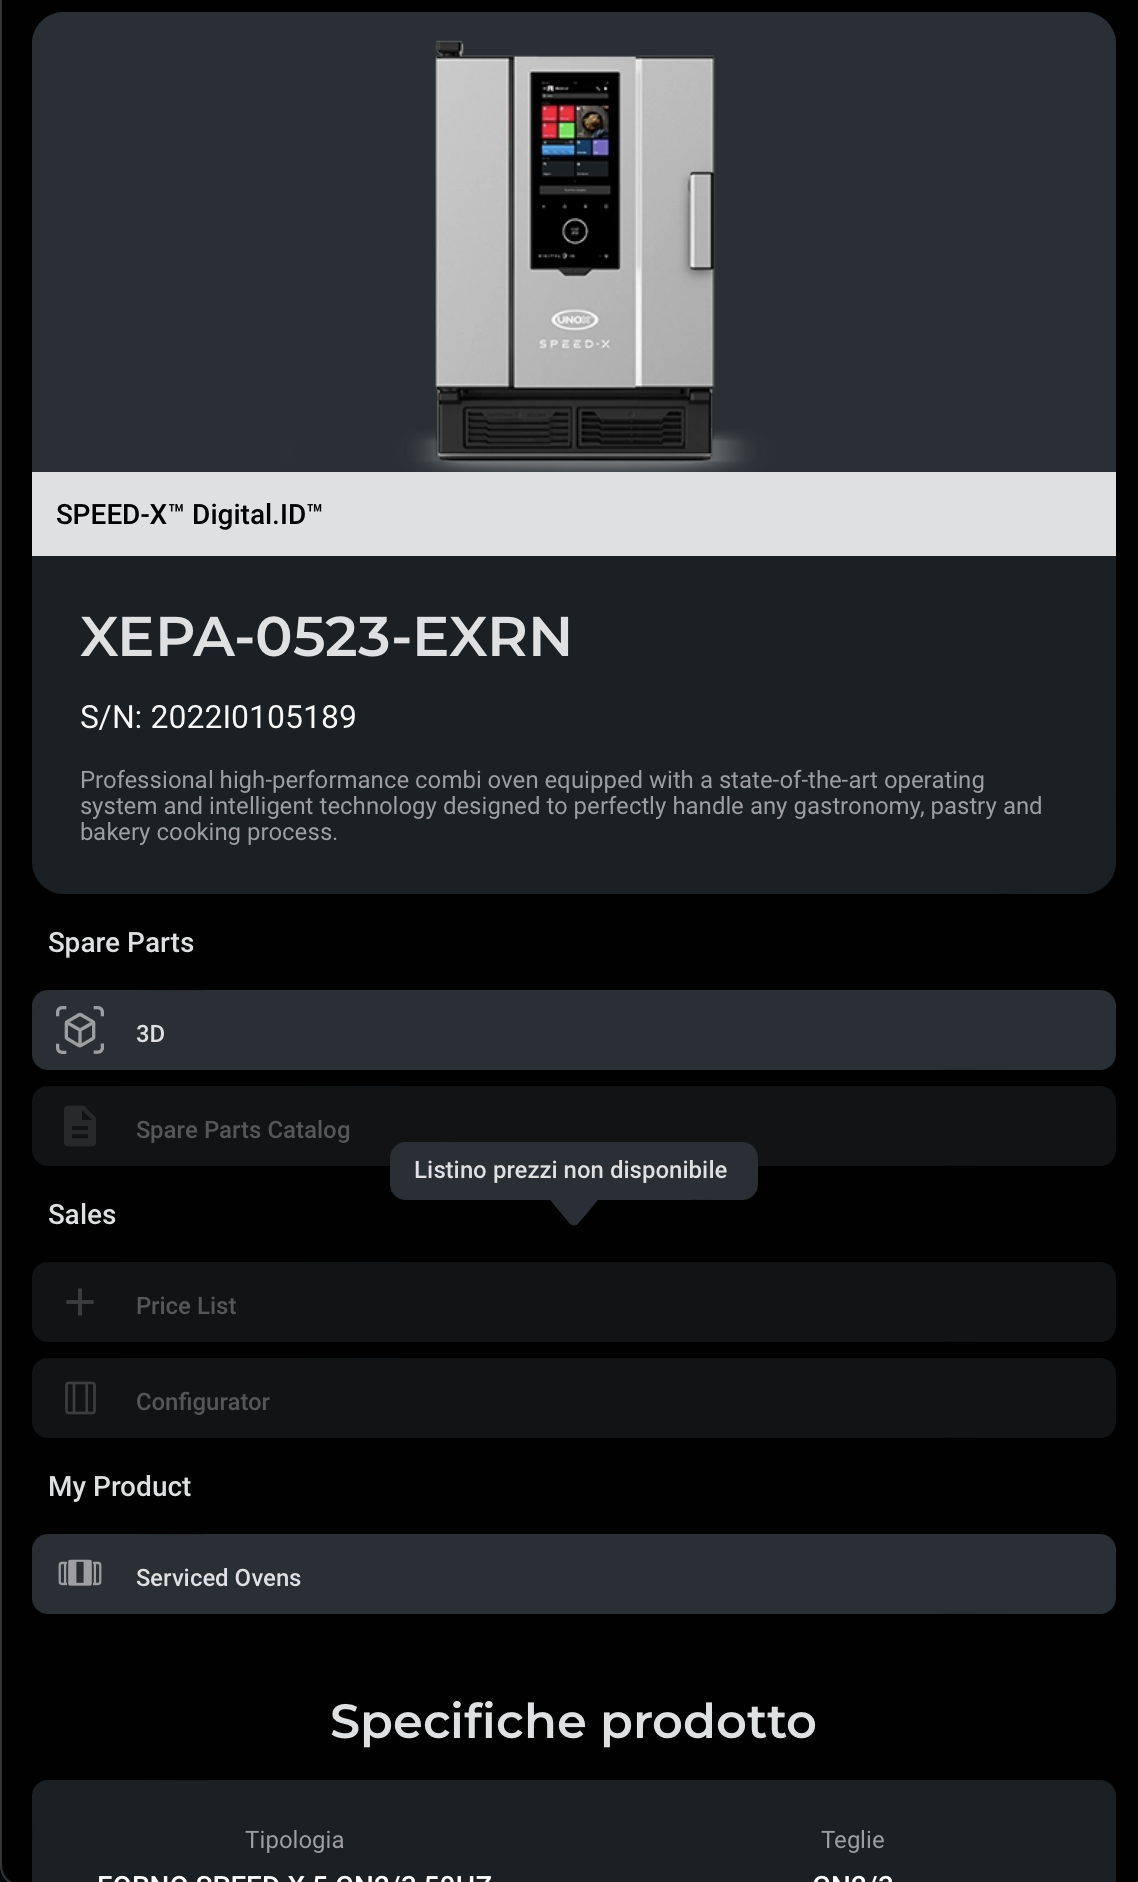
\includegraphics[alt={Screenshot della pagina \textit{"Product Page"} su piattaforma \textit{mobile}}, height=15cm]{img/ProductPageMobile}
    \caption{App \textit{DDC Service} pagina \textit{Product Page} piattaforma \textit{Mobile}}
    \label{fig:productpagemobile}
\end{figure}

La figura presenta la stessa pagina \textit{"Product Page"}, ma su piattaforma \textit{mobile}.
L'applicazione è stata ottimizzata per garantire un'esperienza d'uso eccellente anche su dispositivi \textit{mobile}, con un \textit{design} responsivo che si adatta a diverse dimensioni di schermo.

\begin{figure}[H]
    \centering
    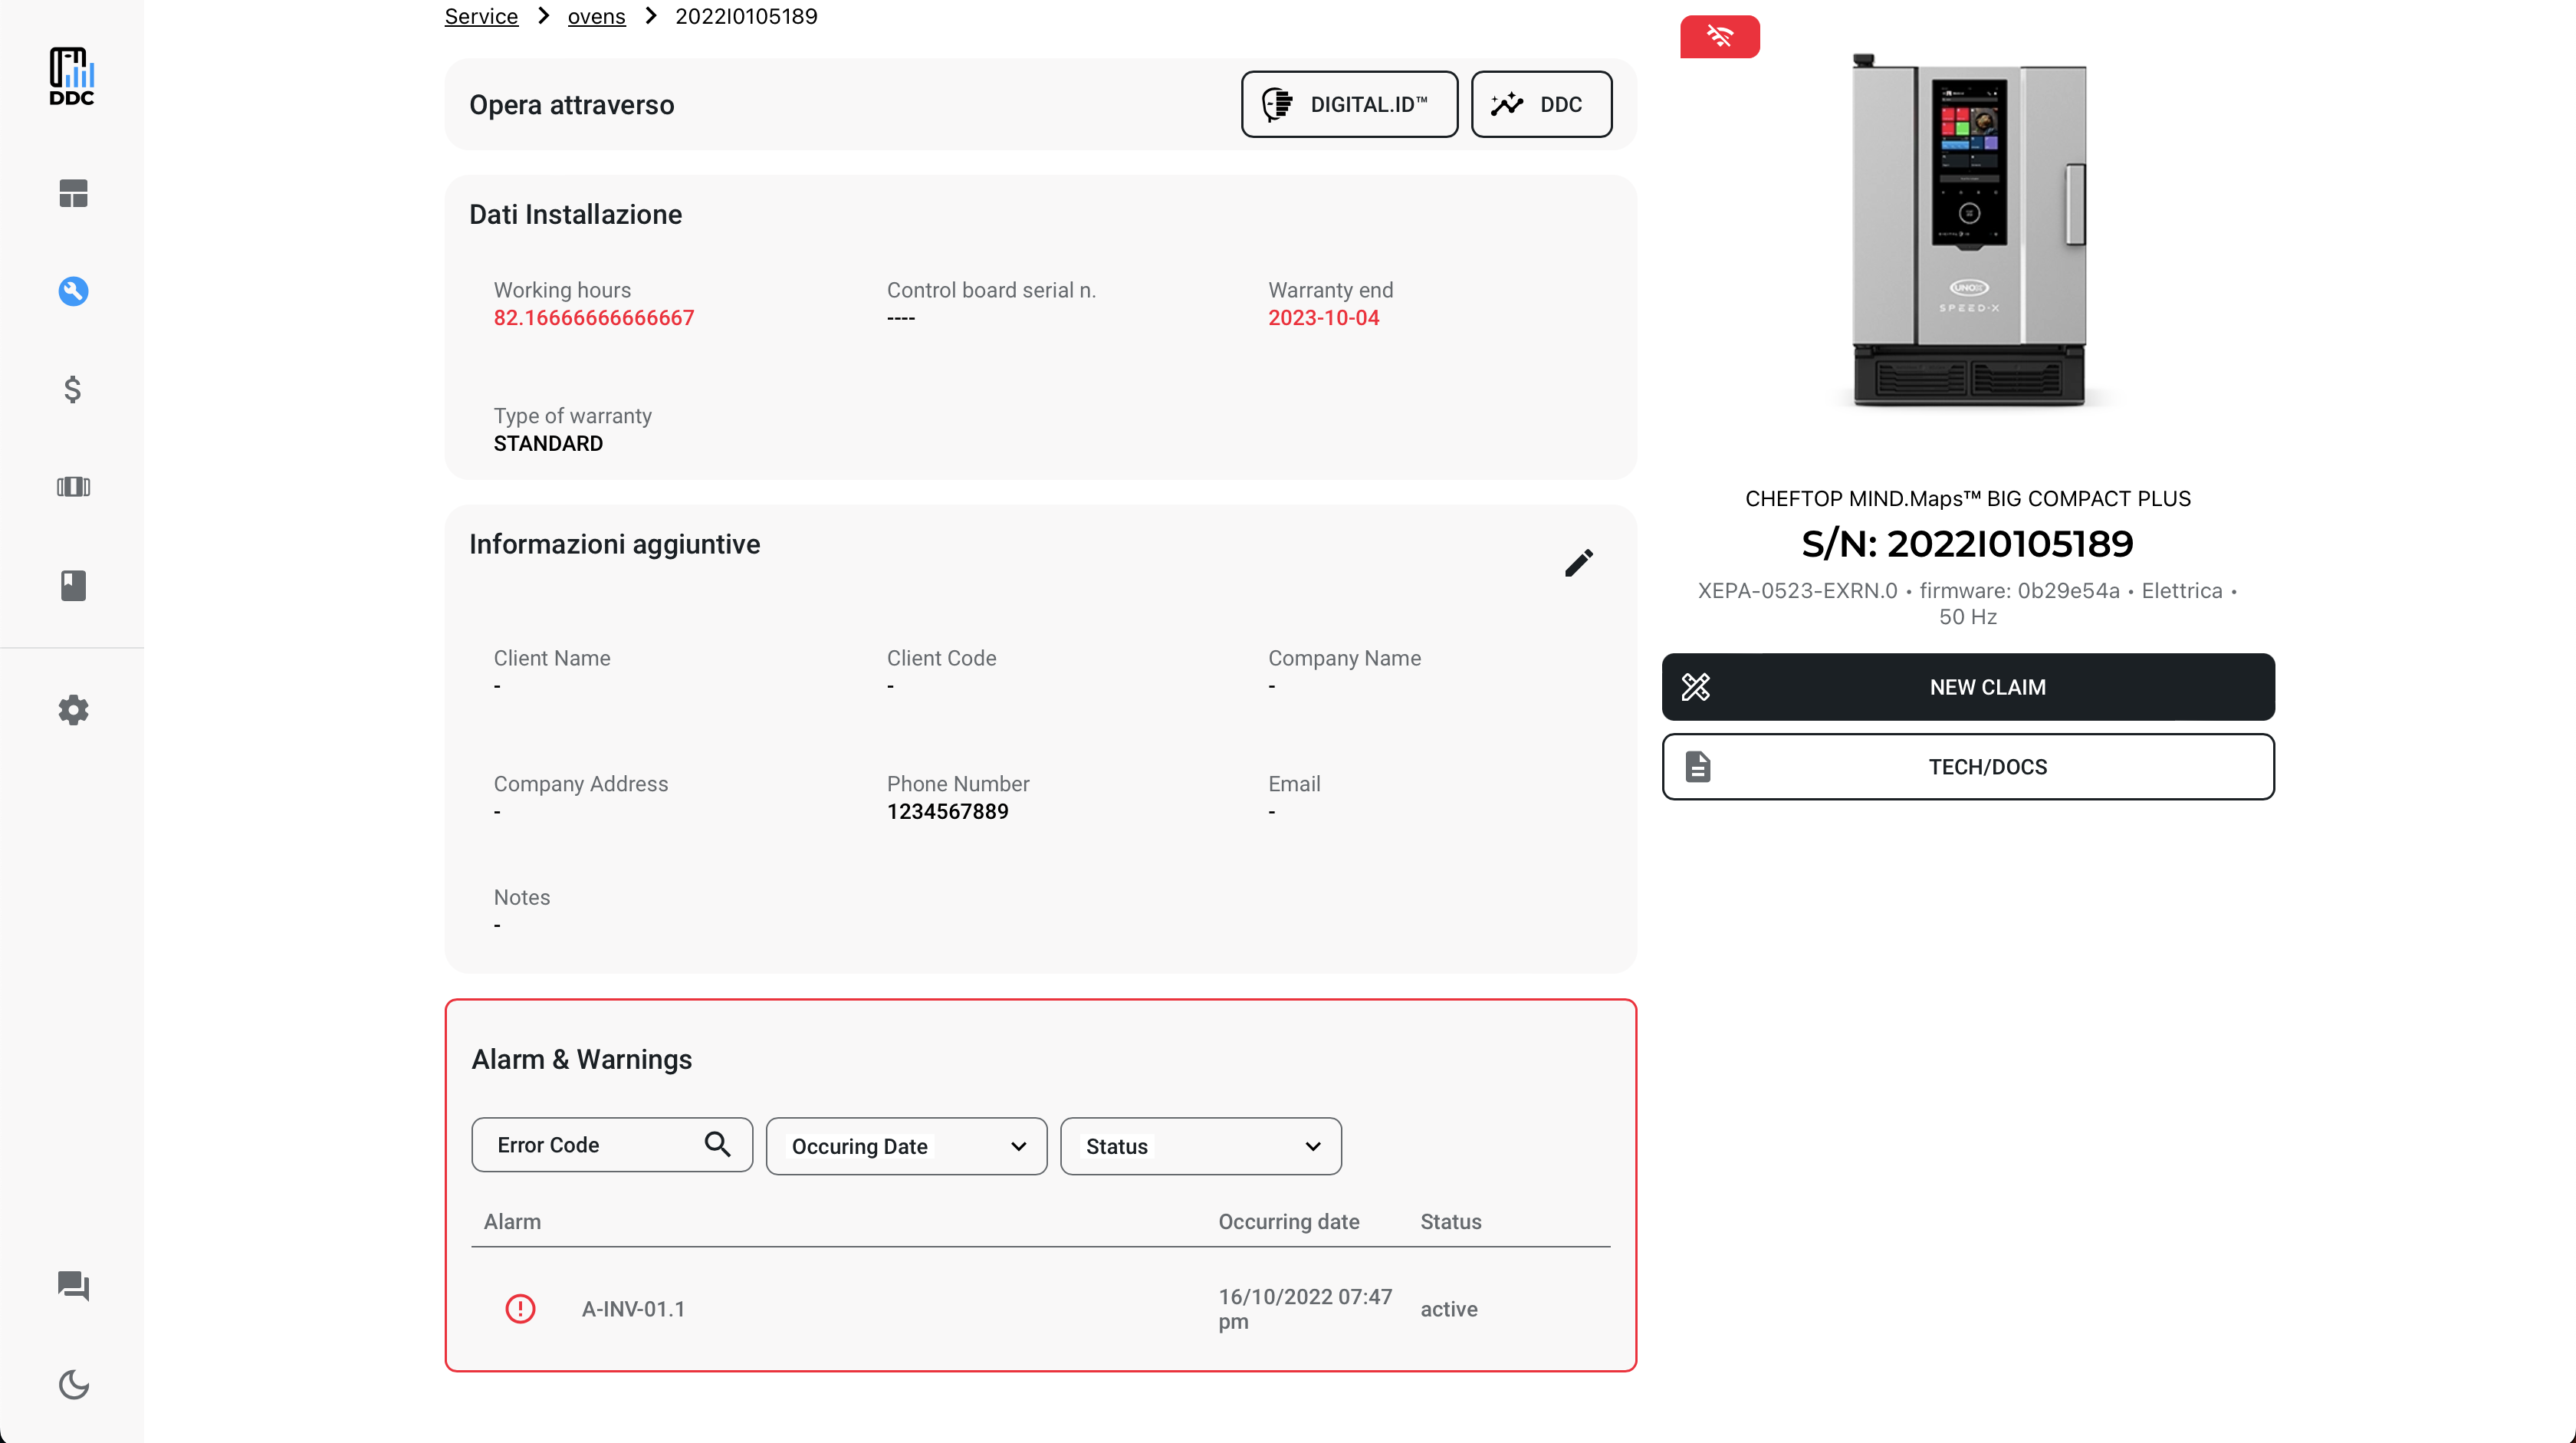
\includegraphics[alt={Screenshot della pagina \textit{"Serviced Oven"} su piattaforma \textit{Web}}, height=10cm]{img/ServicedOvenWeb}
    \caption{App \textit{DDC Service} pagina \textit{Serviced Oven} piattaforma \textit{Web}}
    \label{fig:servicedovenweb}
\end{figure}

La figura \ref{fig:servicedovenweb} illustra la pagina \textit{"Serviced Oven"} sulla piattaforma \textit{Web} dell'applicazione.
Questa pagina permette agli utenti di gestire i forni che necessitano di assistenza.
\section{Conoscenze acquisite}

Durante il mio \textit{stage}, ho avuto l'opportunità di acquisire una vasta gamma di conoscenze e competenze, sia tecniche che organizzative. È stato il mio primo impiego \textit{full-time}, che mi ha dato l'opportunità di acquisire conoscenze sul mondo del lavoro, sulla struttura organizzativa di un'azienda, e sulle attività svolte al suo interno.

\subsection{Competenze Organizzative}

Tra le \textit{soft skill} che sono riuscito a sviluppare durante questo periodo di stage posso enumerare:
\begin{itemize}
    \item \textbf{Gestione del tempo e pianificazione delle attività}: Ho imparato a gestire il mio tempo in modo efficiente e a pianificare le attività per rispettare le scadenze.
    \item \textbf{Collaborazione tra team}: Ho migliorato le mie capacità di comunicazione e di lavoro di squadra, imparando a coordinarmi il lavoro e risolvere i conflitti in modo efficace.
\end{itemize}

È innegabile, però, che molte di più sono state le conoscenze tecniche acquisite in questo periodo.
Di seguito, riporto i principali punti di apprendimento:

\subsection{Gestione delle \textit{Monorepo}}

Uno degli aspetti più significativi del mio lavoro è stato l'apprendimento della gestione delle \gls{monorepog}\glox.
Al giorno d'oggi, l'evoluzione tecnologica è in continua espansione e quello che oggi può essere considerato utile, un domani potrebbe essere considerato \textit{deprecato}.
 Qualsiasi sia il linguaggio di programmazione o il \textit{framework} utilizzato, si parte sempre da un \textit{boilerplate} nei nostri progetti, non capendo realmente cosa quel codice sia o implicitamente imponga.
 Studiare e sapere come funziona una \textit{monorepo} permette di avere gli strumenti per comprendere i progetti e saperli amministrare.
 Nell'ambito dello sviluppo in \textit{Javascript} e in generale con \textit{Node.js}, sapere come gestire le dipendenze in una \textit{monorepo} è una cosa molto importante e questa conoscenza è tra le più importanti che reputo di aver appreso.

Di seguito posso elencare le conoscenze acquisite che reputo più importanti:

\begin{itemize}
    \item \textbf{Centralizzazione delle dipendenze}: Ho appreso i benefici di una centralizzazione delle dipendenze, i vincoli e le sicurezze che garantisce. Questo è particolarmente utile per evitare conflitti e garantire la coerenza tra i vari progetti, oltre che una gestione del \gls{cicdg}\glox migliore.
    \item \textbf{Strumenti di automazione}: Ho imparato a utilizzare strumenti come \textit{Nx}, che facilitano la gestione delle \textit{monorepo} automatizzando compiti comuni come la gestione delle versioni, le pubblicazioni e la condivisione di codice tra i progetti.
\end{itemize}

\subsection{Tecnologie Principali Apprese}

Durante lo stage, ho avuto l'opportunità di lavorare con una serie di tecnologie moderne, migliorando notevolmente le mie competenze tecniche.
La più importante tra tutte è \textit{React} e \textit{React Native} e, in generale, le tecnologie legate allo sviluppo di applicazioni.
Ho imparato a sviluppare utilizzando questa tecnologia, andando nel dettaglio del loro funzionamento e cercando di capire come funzionassero oltre ad utilizzarle e basta.

\begin{itemize}
    \item \textbf{React Native}: Ho approfondito l'uso di \textit{React Native} per lo sviluppo di applicazioni mobili multipiattaforma.
    Ho imparato a creare componenti riutilizzabili, gestire lo stato dell'applicazione con \textit{Redux} e utilizzare \textit{framework} come \textit{Expo}.
    Questa tecnologia mi ha permesso di sviluppare applicazioni efficienti e di alta qualità per diverse piattaforme con una base di codice unica.
    \item \textbf{GraphQL}: Ho acquisito competenze nell'uso di \textit{GraphQL}. Ho imparato i benefici nell'utilizzare questo protocollo di comunicazione nelle \textit{API}.
    \item \textbf{Dripsy/Solito/Moti}: Ho scoperto e utilizzato lo \textit{stack} \textit{Dripsy/Solito/Moti} per la realizzazione di applicazioni multipiattaforma.
    Questo \textit{stack} si è rivelato estremamente utile per gestire con facilità il \textit{routing}, le animazioni e lo stile delle applicazioni.
    \textit{Dripsy} offre una potente libreria per la gestione dello stile in \textit{React Native}, \textit{Solito} facilita il \textit{routing} tra diverse piattaforme e \textit{Moti} semplifica la creazione di animazioni complesse.
\end{itemize}

In sintesi, il mio \textit{stage} è stato estremamente arricchente, permettendomi di acquisire competenze tecniche avanzate e di migliorare le mie capacità organizzative e collaborative.
Queste conoscenze non solo hanno contribuito al successo del progetto di \textit{stage}, ma rappresentano anche un bagaglio prezioso per la mia futura carriera professionale.


\section{Valutazione personale}

Durante il mio percorso di stage, ho avuto modo di mettere in pratica le conoscenze acquisite durante gli studi universitari.
Queste conoscenze mi hanno fornito un solido bagaglio culturale, permettendomi di comprendere e affrontare le sfide del progetto.
Tuttavia, il percorso non è stato privo di difficoltà. Le complessità tecniche e le nuove tecnologie che ho dovuto apprendere hanno reso il lavoro impegnativo, ma estremamente formativo.
I momenti di difficoltà sono stati numerosi, ma proprio grazie a questi ho sviluppato una maggiore persistenza nella risoluzione dei problemi.
Ogni ostacolo superato ha rappresentato un'opportunità di crescita, insegnandomi a non arrendermi di fronte alle sfide e a cercare sempre soluzioni innovative.
L'aspetto più positivo di questa esperienza è stato senza dubbio l'ambiente di lavoro. Ho avuto la fortuna di lavorare in un contesto sereno, dove il rispetto, la collaborazione e il supporto reciproco sono stati fondamentali.
In ogni momento di bisogno, ho potuto contare sull'aiuto di colleghi esperti, che mi hanno guidato e consigliato con professionalità e pazienza.
Il clima lavorativo positivo ha avuto un impatto significativo sulla mia motivazione. Sapere di poter affrontare ogni giornata con serenità mi ha spinto a impegnarmi sempre di più nel progetto, a confrontarmi con i miei colleghi e a continuare a studiare e approfondire le nuove tecnologie.
Questo ambiente mi ha permesso di crescere non solo come professionista, ma anche come individuo, sviluppando una maggiore fiducia nelle mie capacità.
Dal punto di vista educativo, questo stage è stato estremamente prezioso. Ho avuto l'opportunità di lavorare con tecnologie moderne e rilevanti nel mondo del lavoro, ampliando notevolmente il mio bagaglio culturale.
Queste competenze tecniche saranno sicuramente un valore aggiunto per la mia carriera futura, permettendomi di affrontare con maggiore sicurezza e competenza i progetti che verranno.
L'aspetto più importante che questo stage mi ha trasmesso è una nuova capacità di esaminare i problemi e un approccio più pragmatico nell'apprendimento.
Ho imparato a valutare le situazioni in modo critico, a identificare le soluzioni più efficaci e a implementarle.

\pagebreak
In conclusione, posso dire che questa esperienza di stage è stata estremamente positiva. Mi ha permesso di crescere professionalmente e personalmente, offrendomi un'opportunità unica di apprendimento e sviluppo. Sono grato per il supporto ricevuto e per l'ambiente di lavoro stimolante, che mi ha permesso di affrontare con successo le sfide e di acquisire competenze che mi accompagneranno per tutta la vita.


\newpage

    \pagenumbering{roman}
    \backmatter
    \chapter{Bibliografia}
\label{cap:bibliography}

\nocite{*}

% Books bibliography
\printbibliography[heading=subbibliography, title={Testi}, type=book]

% Articles bibliography
\printbibliography[heading=subbibliography, title={Articoli}, type=article]

% Websites bibliography
%\printbibliography[heading=subbibliography, title={Siti}, type=online]

    \chapter{Sitografia}
\label{cap:webliography}
\nocite{*}

% Websites bibliography
\printbibliography[heading=subbibliography, title={\null}, type=online]

\end{document}